% !TeX spellcheck = pl_PL
%%%%%%%%%%%%%%%%%%%%%%%%%%%%%%%%%%%%%%%%%%%
%                                        %
% Szablon pracy dyplomowej magisterskiej %
% zgodny  z aktualnymi  przepisami  SZJK %
%                                        %
%%%%%%%%%%%%%%%%%%%%%%%%%%%%%%%%%%%%%%%%%%
%                                        %
%  (c) Krzysztof Simiński, 2018-2023     %
%                                        %
%%%%%%%%%%%%%%%%%%%%%%%%%%%%%%%%%%%%%%%%%%
%                                        %
% Najnowsza wersja szablonów jest        %
% podstępna pod adresem                  %
% github.com/ksiminski/polsl-aei-theses  %
%                                        %
%%%%%%%%%%%%%%%%%%%%%%%%%%%%%%%%%%%%%%%%%%
%
%
% Projekt LaTeXowy zapewnia odpowiednie formatowanie pracy,
% zgodnie z wymaganiami Systemu zapewniania jakości kształcenia.
% Proszę nie zmieniać ustawień formatowania (np. fontu,
% marginesów, wytłuszczeń, kursywy itd. ).
%
% Projekt można kompilować na kilka sposobów.
%
% 1. kompilacja pdfLaTeX
%
% pdflatex main
% bibtex   main
% pdflatex main
% pdflatex main
%
%
% 2. kompilacja XeLaTeX
%
% Kompilatacja przy użyciu XeLaTeXa różni się tym, że na stronie
% tytułowej używany jest font Calibri. Wymaga to jego uprzedniego
% zainstalowania.
%
% xelatex main
% bibtex  main
% xelatex main
% xelatex main
%
%
%%%%%%%%%%%%%%%%%%%%%%%%%%%%%%%%%%%%%%%%%%%%%%%%%%%%%
% W przypadku pytań, uwag, proszę pisać na adres:   %
%      krzysztof.siminski(małpa)polsl.pl            %
%%%%%%%%%%%%%%%%%%%%%%%%%%%%%%%%%%%%%%%%%%%%%%%%%%%%%
%
% Chcemy ulepszać szablony LaTeXowe prac dyplomowych.
% Wypełniając ankietę spod poniższego adresu pomogą
% Państwo nam to zrobić. Ankieta jest całkowicie
% anonimowa. Dziękujemy!


% https://docs.google.com/forms/d/e/1FAIpQLScyllVxNKzKFHfILDfdbwC-jvT8YL0RSTFs-s27UGw9CKn-fQ/viewform?usp=sf_link
%
%%%%%%%%%%%%%%%%%%%%%%%%%%%%%%%%%%%%%%%%%%%%%%%%%%%%%%%%%%%%%%%%%%%%%%%%%

%%%%%%%%%%%%%%%%%%%%%%%%%%%%%%%%%%%%%%%%%%%%%%%
%                                             %
% PERSONALIZACJA PRACY - DANE PRACY           %
%                                             %
%%%%%%%%%%%%%%%%%%%%%%%%%%%%%%%%%%%%%%%%%%%%%%%

% Proszę wpisać swoje dane w poniższych definicjach.

% TODO
% dane autora
\newcommand{\FirstNameAuthor}{Jakub}
\newcommand{\SurnameAuthor}{Kula}
\newcommand{\IdAuthor}{296849}   % numer albumu  (bez $\langle$ i $\rangle$)

% drugi autor:
%\newcommand{\FirstNameCoauthor}{Imię}   % Jeżeli jest drugi autor, to tutaj należy podać imię.
%\newcommand{\SurnameCoauthor}{Nazwisko} % Jeżeli jest drugi autor, to tutaj należy podać nazwisko.
%\newcommand{\IdCoauthor}{$\langle$wpisać właściwy$\rangle$}  % numer albumu drugiego autora (bez $\langle$ i $\rangle$)
% Gdy nie ma drugiego autora, należy zostawić poniższe definicje puste, jak poniżej. Gdy jest drugi autor, należy zakomentować te linie.
\newcommand{\FirstNameCoauthor}{} % Jeżeli praca ma tylko jednego autora, to dane drugiego autora zostają puste.
\newcommand{\SurnameCoauthor}{}   % Jeżeli praca ma tylko jednego autora, to dane drugiego autora zostają puste.
\newcommand{\IdCoauthor}{}  % Jeżeli praca ma tylko jednego autora, to dane drugiego autora zostają puste.
%%%%%%%%%%

\newcommand{\Supervisor}{dr hab. inż. Pander Tomasz, prof. PŚ}     % dane promotora (bez $\langle$ i $\rangle$)
\newcommand{\Title}{Zastosowanie metod sztucznej inteligencji do detekcji arytmii na podstawie sygnałów PPG}           % tytuł pracy po polsku
\newcommand{\TitleAlt}{Application of artificial intelligence methods for arrhythmia detection based on PPG signal}                     % thesis title in English
\newcommand{\Program}{Informatyka}            % kierunek studiów  (bez $\langle$ i $\rangle$)
\newcommand{\Specialisation}{Internet i technologie sieciowe}     % specjalność  (bez $\langle$ i $\rangle$)
\newcommand{\Departament}{Cybernetyki, Nanotechnologii i Przetwarzania Danych}        % katedra promotora  (bez $\langle$ i $\rangle$)

% Jeżeli został wyznaczony promotor pomocniczy lub opiekun, proszę go/ją wpisać ...
\newcommand{\Consultant}{} % dane promotora pomocniczego, opiekuna (bez $\langle$ i $\rangle$)
% ... w przeciwnym razie proszę zostawić puste miejsce jak poniżej:
%\newcommand{\Consultant}{} % brak promotowa pomocniczego / opiekuna

% koniec fragmentu do modyfikacji
%%%%%%%%%%%%%%%%%%%%%%%%%%%%%%%%%%%%%%%%%%


%%%%%%%%%%%%%%%%%%%%%%%%%%%%%%%%%%%%%%%%%%%%%%%
%                                             %
% KONIEC PERSONALIZACJI PRACY                 %
%                                             %
%%%%%%%%%%%%%%%%%%%%%%%%%%%%%%%%%%%%%%%%%%%%%%%

%%%%%%%%%%%%%%%%%%%%%%%%%%%%%%%%%%%%%%%%


%%%%%%%%%%%%%%%%%%%%%%%%%%%%%%%%%%%%%%%%%%%%%%%
%                                             %
% PROSZĘ NIE MODYFIKOWAĆ PONIŻSZYCH USTAWIEŃ! %
%                                             %
%%%%%%%%%%%%%%%%%%%%%%%%%%%%%%%%%%%%%%%%%%%%%%%



\documentclass[a4paper,twoside,12pt]{book}
\usepackage[utf8]{inputenc}
\usepackage[T1]{fontenc}
\usepackage{amsmath,amsfonts,amssymb,amsthm}
\usepackage[british,polish]{babel}
\usepackage{indentfirst}
\usepackage{xurl}
\usepackage{xstring}
\usepackage{ifthen}

\usepackage{makecell}
\usepackage{siunitx}
\usepackage{tikz}
\usetikzlibrary{arrows.meta, positioning, shapes.geometric}

\usepackage{ifxetex}

\ifxetex
	\usepackage{fontspec}
	\defaultfontfeatures{Mapping=tex-text} % to support TeX conventions like ``--''
	\usepackage{xunicode} % Unicode support for LaTeX character names (accents, European chars, etc)
	\usepackage{xltxtra} % Extra customizations for XeLaTeX
\else
	\usepackage{lmodern}
\fi



\usepackage[margin=2.5cm]{geometry}
\usepackage{graphicx}
\usepackage{hyperref}
\usepackage{booktabs}
\usepackage{tikz}
\usepackage{pgfplots}
\usepackage{mathtools}
\usepackage{geometry}
\usepackage{subcaption}   % subfigures
\usepackage[page]{appendix} % toc,
\renewcommand{\appendixtocname}{Dodatki}
\renewcommand{\appendixpagename}{Dodatki}
\renewcommand{\appendixname}{Dodatek}

\usepackage{csquotes}
\usepackage[natbib=true,backend=bibtex,maxbibnames=99,sorting=none]{biblatex}  % kompilacja bibliografii BibTeXem
%\usepackage[natbib=true,backend=biber,maxbibnames=99]{biblatex}  % kompilacja bibliografii Biberem
\bibliography{biblio}

\usepackage{ifmtarg}   % empty commands  

\usepackage{setspace}
\onehalfspacing


\frenchspacing



%%%% TODO LIST GENERATOR %%%%%%%%%

\usepackage{color}
\definecolor{brickred}      {cmyk}{0   , 0.89, 0.94, 0.28}

\makeatletter \newcommand \kslistofremarks{\section*{Uwagi} \@starttoc{rks}}
\newcommand\l@uwagas[2]
{\par\noindent \textbf{#2:} %\parbox{10cm}
	{#1}\par} \makeatother



\newcommand{\ksremark}[1]{%
	{%\marginpar{\textdbend}
			{\color{brickred}{[#1]}}}%
	\addcontentsline{rks}{uwagas}{\protect{#1}}%
}

\newcommand{\comma}{\ksremark{przecinek}}
\newcommand{\nocomma}{\ksremark{bez przecinka}}
\newcommand{\styl}{\ksremark{styl}}
\newcommand{\ortografia}{\ksremark{ortografia}}
\newcommand{\fleksja}{\ksremark{fleksja}}
\newcommand{\pauza}{\ksremark{pauza `--', nie dywiz `-'}}
\newcommand{\kolokwializm}{\ksremark{kolokwializm}}
\newcommand{\cudzyslowy}{\ksremark{,,polskie cudzysłowy''}}

%%%%%%%%%%%%%% END OF TODO LIST GENERATOR %%%%%%%%%%%

\newcommand{\printCoauthor}{%		
	\StrLen{\FirstNameCoauthor}[\FNCoALen]
	\ifthenelse{\FNCoALen > 0}%
	{%
		{\large\bfseries\Coauthor\par}

			{\normalsize\bfseries \LeftId: \IdCoauthor\par}
	}%
	{}
}

%%%%%%%%%%%%%%%%%%%%%
\newcommand{\autor}{%		
	\StrLen{\FirstNameCoauthor}[\FNCoALenXX]
	\ifthenelse{\FNCoALenXX > 0}%
	{\FirstNameAuthor\ \SurnameAuthor, \FirstNameCoauthor\ \SurnameCoauthor}%
	{\FirstNameAuthor\ \SurnameAuthor}%
}
%%%%%%%%%%%%%%%%%%%%%

\StrLen{\FirstNameCoauthor}[\FNCoALen]
\ifthenelse{\FNCoALen > 0}%
{%
	\author{\FirstNameAuthor\ \SurnameAuthor, \FirstNameCoauthor\ \SurnameCoauthor}
}%
{%
	\author{\FirstNameAuthor\ \SurnameAuthor}
}%

%%%%%%%%%%%% ZYWA PAGINA %%%%%%%%%%%%%%%
% brak kapitalizacji zywej paginy
\usepackage{fancyhdr}
\pagestyle{fancy}
\fancyhf{}
\fancyhead[LO]{\nouppercase{\it\rightmark}}
\fancyhead[RE]{\nouppercase{\it\leftmark}}
\fancyhead[LE,RO]{\it\thepage}


\fancypagestyle{tylkoNumeryStron}{%
	\fancyhf{}
	\fancyhead[LE,RO]{\it\thepage}
}

\fancypagestyle{bezNumeracji}{%
	\fancyhf{}
	\fancyhead[LE,RO]{}
}


\fancypagestyle{NumeryStronNazwyRozdzialow}{%
	\fancyhf{}
	\fancyhead[LE]{\nouppercase{\autor}}
	\fancyhead[RO]{\nouppercase{\leftmark}}
	\fancyfoot[CE, CO]{\thepage}
}


%%%%%%%%%%%%% OBCE WTRETY  
\newcommand{\obcy}[1]{\emph{#1}}
\newcommand{\english}[1]{{\selectlanguage{british}\obcy{#1}}}
%%%%%%%%%%%%%%%%%%%%%%%%%%%%%

% polskie oznaczenia funkcji matematycznych
\renewcommand{\tan}{\operatorname {tg}}
\renewcommand{\log}{\operatorname {lg}}

% jeszcze jakies drobiazgi

\newcounter{stronyPozaNumeracja}

%%%%%%%%%%%%%%%%%%%%%%%%%%% 
\newcommand{\printOpiekun}[1]{%		

	\StrLen{\Consultant}[\mystringlen]
	\ifthenelse{\mystringlen > 0}%
	{%
		{\large{\bfseries OPIEKUN, PROMOTOR POMOCNICZY}\par}

			{\large{\bfseries \Consultant}\par}
	}%
	{}
}
%
%%%%%%%%%%%%%%%%%%%%%%%%%%%%%%%%%%%%%%%%%%%%%%

% Proszę nie modyfikować poniższych definicji!
\newcommand{\Author}{\FirstNameAuthor\ \MakeUppercase{\SurnameAuthor}}
\newcommand{\Coauthor}{\FirstNameCoauthor\ \MakeUppercase{\SurnameCoauthor}}
\newcommand{\Type}{PRACA MAGISTERSKA}
\newcommand{\Faculty}{Wydział Automatyki, Elektroniki i Informatyki}
\newcommand{\Polsl}{Politechnika Śląska}
\newcommand{\Logo}{politechnika_sl_logo_bw_pion_pl.pdf}
\newcommand{\LeftId}{Nr albumu}
\newcommand{\LeftProgram}{Kierunek}
\newcommand{\LeftSpecialisation}{Specjalność}
\newcommand{\LeftSUPERVISOR}{PROWADZĄCY PRACĘ}
\newcommand{\LeftDEPARTMENT}{KATEDRA}
%%%%%%%%%%%%%%%%%%%%%%%%%%%%%%%%%%%%%%%%%%%%%%

%%%%%%%%%%%%%%%%%%%%%%%%%%%%%%%%%%%%%%%%%%%%%%%
%                                             %
% KONIEC USTAWIEŃ                             %
%                                             %
%%%%%%%%%%%%%%%%%%%%%%%%%%%%%%%%%%%%%%%%%%%%%%%




%%%%%%%%%%%%%%%%%%%%%%%%%%%%%%%%%%%%%%%%%%%%%%%
%                                             %
% MOJE PAKIETY, USTAWIENIA ITD                %
%                                             %
%%%%%%%%%%%%%%%%%%%%%%%%%%%%%%%%%%%%%%%%%%%%%%%

% Tutaj proszę umieszczać swoje pakiety, makra, ustawienia itd.



%%%%%%%%%%%%%%%%%%%%%%%%%%%%%%%%%%%%%%%%%%%%%%%%%%%%%%%%%%%%%%%%%%%%%
% listingi i fragmentu kodu źródłowego 
% pakiet: listings lub minted
% % % % % % % % % % % % % % % % % % % % % % % % % % % % % % % % % % % 

% biblioteka listings
\usepackage{listings}
\lstset{%
	morekeywords={string,exception,std,vector},% słowa kluczowe rozpoznawane przez pakiet listings
	language=C++,% C, Matlab, Python, SQL, TeX, XML, bash, ... - vide https://www.ctan.org/pkg/listings
	commentstyle=\textit,%
	identifierstyle=\textsf,%
	keywordstyle=\sffamily\bfseries, %\texttt, %
	%captionpos=b,%
	tabsize=3,%
	frame=lines,%
	numbers=left,%
	numberstyle=\tiny,%
	numbersep=5pt,%
	breaklines=true,%
	escapeinside={@*}{*@},%
}

% % % % % % % % % % % % % % % % % % % % % % % % % % % % % % % % % % % 
% pakiet minted
%\usepackage{minted}

% pakiet wymaga specjalnego kompilowania:
% pdflatex -shell-escape main.tex
% xelatex  -shell-escape main.tex

%\usepackage[chapter]{minted} % [section]
%%\usemintedstyle{bw}   % czarno-białe kody 
%
%\setminted % https://ctan.org/pkg/minted
%{
%%fontsize=\normalsize,%\footnotesize,
%%captionpos=b,%
%tabsize=3,%
%frame=lines,%
%framesep=2mm,
%numbers=left,%
%numbersep=5pt,%
%breaklines=true,%
%escapeinside=@@,%
%}

%%%%%%%%%%%%%%%%%%%%%%%%%%%%%%%%%%%%%%%%%%%%%%%%%%%%%%%%%%%%%%%%%%%%%



%%%%%%%%%%%%%%%%%%%%%%%%%%%%%%%%%%%%%%%%%%%%%%%
%                                             %
% KONIEC MOICH USTAWIEŃ                       %
%                                             %
%%%%%%%%%%%%%%%%%%%%%%%%%%%%%%%%%%%%%%%%%%%%%%%



%%%%%%%%%%%%%%%%%%%%%%%%%%%%%%%%%%%%%%%%
\usepackage{array}
\usepackage{makecell}
\renewcommand{\arraystretch}{1.5}

\begin{document}
%\kslistofremarks

\frontmatter

%%%%%%%%%%%%%%%%%%%%%%%%%%%%%%%%%%%%%%%%%%%%%%%
%                                             %
% PROSZĘ NIE MODYFIKOWAĆ STRONY TYTUŁOWEJ!    %
%                                             %
%%%%%%%%%%%%%%%%%%%%%%%%%%%%%%%%%%%%%%%%%%%%%%%


%%%%%%%%%%%%%%%%%%  STRONA TYTUŁOWA %%%%%%%%%%%%%%%%%%%
\pagestyle{empty}
{
	\newgeometry{top=1.5cm,%
		bottom=2.5cm,%
		left=3cm,
		right=2.5cm}

	\ifxetex
		\begingroup
		\setsansfont{Calibri}

	\fi
	\sffamily
	\begin{center}
		\includegraphics[width=50mm]{\Logo}


		{\Large\bfseries\Type\par}

		\vfill  \vfill

		{\large\Title\par}

		\vfill

		{\large\bfseries\Author\par}

		{\normalsize\bfseries \LeftId: \IdAuthor}

		\printCoauthor

		\vfill

		{\large{\bfseries \LeftProgram:} \Program\par}

		{\large{\bfseries \LeftSpecialisation:} \Specialisation\par}

		\vfill  \vfill 	\vfill 	\vfill 	\vfill 	\vfill 	\vfill

		{\large{\bfseries \LeftSUPERVISOR}\par}

		{\large{\bfseries \Supervisor}\par}

		{\large{\bfseries \LeftDEPARTMENT\ \Departament} \par}

		{\large{\bfseries \Faculty}\par}

		\vfill  \vfill


		\printOpiekun{\Consultant}

		\vfill  \vfill

		{\large\bfseries  Gliwice \the\year}

	\end{center}
	\ifxetex
		\endgroup
	\fi
	\restoregeometry
}

%%%%%%%%%%%%%%%%%%%%%%%%%%%%%%%%%%%%%%%%%%%%%%%
%                                             %
% KONIEC STRONY TYTUŁOWEJ                     %
%                                             %
%%%%%%%%%%%%%%%%%%%%%%%%%%%%%%%%%%%%%%%%%%%%%%%  


\cleardoublepage

\rmfamily\normalfont
\pagestyle{empty}


%%% No to zaczynamy pisać pracę :-) %%%%

% TODO
\subsubsection*{Tytuł pracy}
\Title

\subsubsection*{Streszczenie}
(Streszczenie pracy - odpowiednie pole w systemie APD powinno zawierać kopię tego streszczenia.)

\subsubsection*{Słowa kluczowe}
(2-5 slow (fraz) kluczowych, oddzielonych przecinkami)

\subsubsection*{Thesis title}
\begin{otherlanguage}{british}
	\TitleAlt
\end{otherlanguage}

\subsubsection*{Abstract}
\begin{otherlanguage}{british}
	(Thesis abstract - to be copied into an appropriate field during an electronic submission - in English.)
\end{otherlanguage}
\subsubsection*{Key words}
\begin{otherlanguage}{british}
	(2-5 keywords, separated by commas)
\end{otherlanguage}




%%%%%%%%%%%%%%%%%% SPIS TRESCI %%%%%%%%%%%%%%%%%%%%%%
% Add \thispagestyle{empty} to the toc file (main.toc), because \pagestyle{empty} doesn't work if the TOC has multiple pages
\addtocontents{toc}{\protect\thispagestyle{empty}}
\tableofcontents

%%%%%%%%%%%%%%%%%%%%%%%%%%%%%%%%%%%%%%%%%%%%%%%%%%%%%
\setcounter{stronyPozaNumeracja}{\value{page}}
\mainmatter
\pagestyle{empty}

\cleardoublepage

\pagestyle{NumeryStronNazwyRozdzialow}

%%%%%%%%%%%%%% wlasciwa tresc pracy %%%%%%%%%%%%%%%%%

% TODO
\chapter{Wstęp}
\section{Cel i zakres pracy}
\section{Aktualny stan wiedzy}
\section{Charakterystyka rozdziałów}

% TODO

\chapter{Charakterystyka arytmii serca i sygnału PPG}
\section{Klasyfikacja i mechanizmy arytmii serca}
\subsection{Arytmie nadkomorowe}
\subsection{Arytmie komorowe}
\subsection{Migotanie przedsionków}
\section{Fotopletyzmografia - zasada działania i zastosowania}

\chapter{Metody uczenia maszynowego}
\section{Klasyczne metody}

\subsection*{Metoda najbliższych sąsiadów (KNN)}
Klasyfikator opierający swoje predykcje na analizie $k$ najbliższych sąsiadów ze zbioru treningowego. Metoda ta wykorzystuje metryki odległości do wyznaczenia próbek najbardziej zbliżonych do klasyfikowanego punktu, a następnie przypisuje mu etykietę tej klasy, która najczęściej występuje wśród wybranych $k$ sąsiadów.

Najczęściej stosowaną metryką odległości jest odległość euklidesowa, zdefiniowana wzorem:
\begin{equation}
	d(x, y) = \left( \sum_{i=1}^{n} |x_i - y_i|^{2} \right)^{\frac{1}{2}}
\end{equation}
gdzie $x = (x_1, x_2, \ldots, x_n)$ oraz $y = (y_1, y_2, \ldots, y_n)$ to dwa punkty w $n$-wymiarowej przestrzeni cech. Generalizacją odległości Euklidesowej jest odległości Minkowskiego zdefiniowana jako:
\begin{equation}
	d(x, y) = \left( \sum_{i=1}^{n} |x_i - y_i|^{q} \right)^{\frac{1}{q}}
\end{equation}
gdzie q>0 \cite{liu2007web}. Można zauważyc, że dla q=2 otrzymuje odległość Euklidesową, a dla q=1 odległość Manhatan.
Ze względu na to, że algorytm KNN opiera się na obliczaniu odległości między próbkami, istotne jest zachowanie jednolitej skali cech. W przypadku, gdy poszczególne cechy mają różne zakresy wartości, cecha o największej rozpiętości może zdominować obliczenia odległości, a tym samym nieproporcjonalnie wpłynąć na wynik predykcji.

W przypadku tego klasyfikatora kluczowe jest odpowiednie dobranie liczby sąsiadów. Zbyt mała wartość parametru k może prowadzić do przeuczenia, w którym model nadmiernie dopasowuje się do danych treningowych i traci zdolność generalizacji. Z kolei zbyt duża liczba sąsiadów skutkuje zjawiskiem niedouczenia, w którym model nie jest w stanie uchwycić istotnych zależności w danych\cite{kuhn2013applied}.

\subsection*{Drzewo decyzyjne}
Model drzewa decyzyjnego opiera się na zagnieżdżonych regułach typu „jeżeli-wtedy”, które dzielą przestrzeń cech na coraz mniejsze podobszary. Struktura drzewa składa się z:
\begin{itemize}
	\item korzenia - punktu początkowego, od którego rozpoczyna się proces podejmowania decyzji,
	\item węzłów decyzyjnyc - zawierających testy logiczne dzielące dane na podzbiory na podstawie wartości cech,
	\item gałęzi - reprezentujących możliwe wyniki testów prowadzące do kolejnych węzłów,
	\item liści - końcowych węzłów, w których przypisywana jest wartość przewidywanej klasy.
\end{itemize}
Proces uczenia drzewa decyzyjnego polega na iteracyjnym wyborze cech oraz odpowiadających im wartości progowych, które najlepiej rozdzielają dane.

\begin{figure}[!h]
	\centering
	\caption{Przykład drzewa decyzyjnego}
	\resizebox{\textwidth}{!}{
		\begin{tikzpicture}[
				edge from parent/.style={draw, -latex},
				level distance=2.8cm,
				sibling distance=6.5cm,
				every node/.style={rectangle, draw, minimum width=3cm, minimum height=1.2cm, align=center, font=\small},
				edge label/.style={font=\small, midway, fill=white}
			]
			\node {Dochód miesięczny \\ > 7000 zł?}
			child {
					node {Liczba produktów \\ > 3?}
					child {
							node {Klasa: \\ Klient lojalny}
							edge from parent node[draw=none, fill=none, left,xshift=15pt] {tak}
						}
					child {
							node {Czas z kontem \\ > 2 lata?}
							edge from parent node[draw=none, fill=none, left, xshift=15pt] {nie}
						}
					edge from parent node[draw=none, fill=none, left,xshift=15pt] {tak}
				}
			child {
					node {Wiek \\ < 30 lat?}
					child {
							node {Czas z kontem \\ > 2 lata?}
							child {
									node {Klasa: \\ Klient okazjonalny}
									edge from parent node[draw=none, fill=none, left, xshift=15pt] {tak}
								}
							child {
									node {Klasa: \\ Klient niska wartość}
									edge from parent node[draw=none, fill=none, right, xshift=-15pt] {nie}
								}
							edge from parent node[draw=none, fill=none, right,xshift=-15pt] {tak}
						}
					child {
							node {Klasa: \\ Klient niska wartość}
							edge from parent node[draw=none, fill=none, right,xshift=-15pt] {nie}
						}
					edge from parent node[draw=none, fill=none, right,xshift=-15pt] {nie}
				};
		\end{tikzpicture}
	}
\end{figure}

Drzewa decyzyjne, dzięki prostocie procesu uczenia i działania, cechują się wysoką interpretowalnością. Mimo że drzewo może zawierać wiele węzłów decyzyjnych, użytkownik jest w stanie z łatwością prześledzić krok po kroku ciąg decyzji prowadzących do końcowej predykcji.
Największą wadą drzew decyzyjnych jest ich skłonność do przeuczania, co oznacza, że model traci zdolność do uogólniania i zbyt dokładnie dopasowuje się do danych ze zbioru uczącego. Zjawisko to szczególnie często występuje w przypadku bardzo rozbudowanych drzew.\\

Podczas procesu budowy drzewa decyzyjnego możliwe jest pełne kontrolowanie jego struktury poprzez określenie między innymi ograniczeń związanych z maksymalną głębokością drzewa oraz minimalną liczbą próbek wymaganą do utworzenia węzła decyzyjnego. Pozwala to na regulację złożoności modelu i ograniczenie ryzyka przeuczenia.
\subsection*{Las losowy}
Klasyfikator oparty na zbiorze drzew decyzyjnych, których predykcje są agregowane w celu podjęcia decyzji końcowej, zwykle przez głosowanie większościowe. Model ten wykorzystuje dwa kluczowe mechanizmy w procesie uczenia:

\begin{itemize}
	\item Bootstrap aggregation - dla każdego drzewa decyzyjnego generowany jest losowy podzbiór próbek (z powtórzeniami) ze zbioru treningowego.
	\item Losowy wybór cech - na każdym etapie podziału drzewa rozważana jest tylko losowo wybrana podgrupa cech.
\end{itemize}

Zastosowanie powyższych technik sprawia, że lasy losowe cechują się większą odpornością na przeuczenie w porównaniu do pojedynczych drzew decyzyjnych. Dodatkową zaletą jest możliwość oszacowania niepewności predykcji na podstawie rozrzutu odpowiedzi poszczególnych drzew. Wadą tej metody jest natomiast ograniczona interpretowalność oraz zwiększone wymagania obliczeniowe i pamięciowe względem pojedynczych modeli drzewiastych.
\subsection*{Naiwny klasyfikator Bayesa}
Klasyfikator oparty na teorii Bayesa, który dokonuje klasyfikacji poprzez ocenę prawdopodobieństwa przynależności wektora cech do poszczególnych klas. Model ten nie analizuje bezpośrednich zależności między cechami a klasą, lecz na podstawie danych treningowych estymuje rozkłady prawdopodobieństwa cech w każdej klasie. Przy klasyfikacji nowych próbek oblicza się prawdopodobieństwo przynależności wektora cech do każdej klasy, a przypisanie następuje do klasy o największym prawdopodobieństwie. Regułę Bayesa można zapisać wzorem:
\begin{equation}
	P(C_k \mid \mathbf{x}) = \frac{P(\mathbf{x} \mid C_k) \cdot P(C_k)}{P(\mathbf{x})},
\end{equation}
gdzie:
\begin{itemize}
	\item $\mathbf{x}$ - wektor cech opisujących próbkę,
	\item $C_k$ - klasa, do której próbka może należeć,
	\item $P(C_k \mid \mathbf{x})$ - prawdopodobieństwo, że próbka o cechach $\mathbf{x}$ należy do klasy $C_k$,
	\item $P(\mathbf{x} \mid C_k)$ - prawdopodobieństwo zaobserwowania cech $\mathbf{x}$, pod warunkiem, że próbka należy do klasy $C_k$,
	\item $P(C_k)$ - prawdopodobieństwo wystąpienia klasy $C_k$,
	\item $P(\mathbf{x})$ - całkowite prawdopodobieństwo wystąpienia cech $\mathbf{x}$.
\end{itemize}

Klasyfikator nazywany jest „naiwnym” ze względu na przyjęte założenie o niezależności cech, które znacząco uproszczają obliczenia statystyczne, jednak jest jest ono zazwyczaj nierealistyczne.

% \begin{figure}[!htbp]
% 	\centering
% 	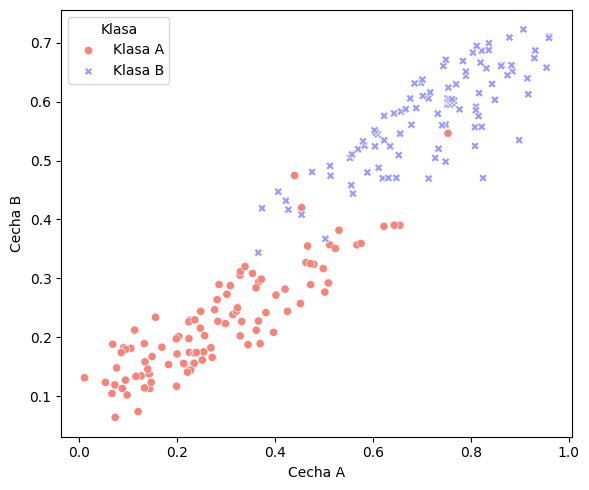
\includegraphics[width=0.5\linewidth]{img/r3/bayes_1.png}
% 	\caption{Przykładowy rozkład klas}
% 	\label{fig:wykres_przyk_roz_klas}
% \end{figure}
% Na przykładzie rozkładu klas względem dwóch cech: A oraz B, przedstawionym na rysunku \ref{fig:wykres_przyk_roz_klas}, można zaobserwować, iż klasy nie są separowalne liniowo - nie istnieje hiperpłaszczyzna, która umożliwiłaby pełne rozdzielenie próbek obu klas bez błędów klasyfikacji. Ponadto, liczebność próbek w obu klasach jest równa, co implikuje, że ich prawdopodobieństwo wylosowania każdej próbki jest jednakowe: $P(A) = P(B)$. W związku z tym że całkowite prawdopodobieństwo wystąpienia cech X jest równe w przypadku klasy A i B, możemy je pominać. Aby ocenić prawdopodobieństwo przynależności nowej próbki wykorzystując teorie Bayesowską, wymagane jest obliczenie rozkładu gęstości klas obu cech.

% \begin{figure}[!htbp]
% 	\centering
% 	\begin{subfigure}[b]{0.45\textwidth}
% 		\centering
% 		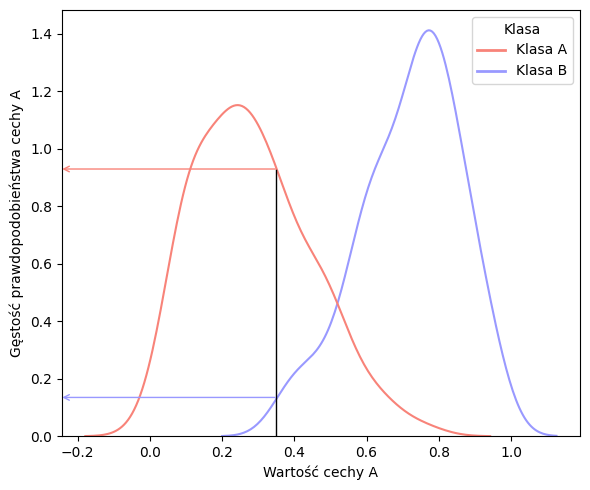
\includegraphics[width=\linewidth]{img/r3/bayes_2.png}
% 		\caption{Rozkład gęstości cechy A}
% 		\label{fig:wykres2}
% 	\end{subfigure}
% 	\hfill
% 	\begin{subfigure}[b]{0.45\textwidth}
% 		\centering
% 		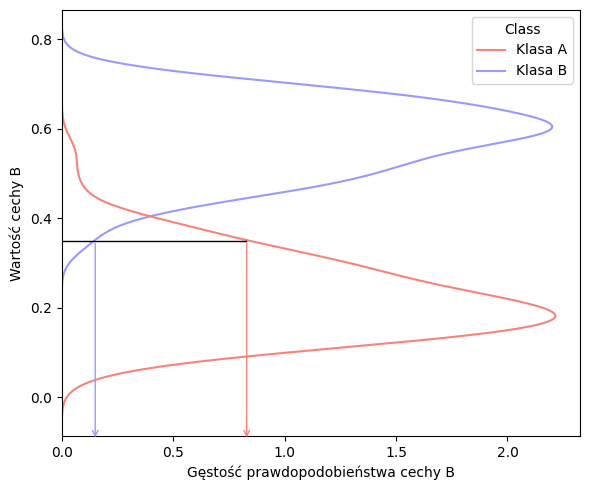
\includegraphics[width=\linewidth]{img/r3/bayes_3.png}
% 		\caption{Rozkład gęstości cechy B}
% 		\label{fig:wykres3}
% 	\end{subfigure}

% 	\caption{Rozkłady gęstości cech w klasach}
% 	\label{fig:subplots_three}
% \end{figure}
% Analizując wykresy przedstawione na rysunku \ref{fig:subplots_three}, można zauważyć, że w rozpatrywanym przypadku rozkłady obu klas wykazują wyraźne różnice względem wartości cech. Dla obu cech, próbki należące do klasy A częściej występują przy niższych wartościach, natomiast próbki klasy B dominują w zakresie wyższych wartości. W przypadku cechy A, punkt przecięcia gęstości rozkładów obu klas - odpowiadający wartości, dla której prawdopodobieństwa przynależności do obu klas są równe - występuje w przybliżeniu przy wartości 0,55. Analogiczny punkt równowagi dla cechy B przypada na wartość około 0,4.

% W celu sprawdzenia porówniania prawdopodobieństwa zdecydowano się sprawdzić prawdopodobieńśtwo przynależności do obu klas dla cech (A,B)=(0.35,0.35)
% \begin{equation}
% 	P((0.35,0.35)\mid A) = 0,
% \end{equation}
% \newpage

\subsection*{Maszyna wektorów nośnych (SVM)}
Maszyna wektorów nośnych to klasyfikator, którego celem jest wyznaczenie optymalnej granicy decyzyjnej oddzielającej dane należące do różnych klas. W sytuacji, gdy dane są liniowo separowalne, istnieje nieskończenie wiele możliwych hiperpłaszczyzn rozdzielających. SVM wybiera tę, która maksymalizuje tzw. margines, czyli minimalną odległość między granicą decyzyjną a najbliższymi punktami obu klas. Takie podejście zapewnia dobrą generalizację klasyfikatora.

W przypadku, gdy dane nie są liniowo separowalne, stosuje się funkcję jądra, która przekształca przestrzeń cech do przestrzeni o wyższym wymiarze, w której możliwe jest liniowe rozdzielenie danych. Wykorzystanie funkcji jądra pozwala SVM na modelowanie nieliniowych granic decyzyjnych bez jawnego przekształcania danych.

\begin{figure}[!h]
	\centering
	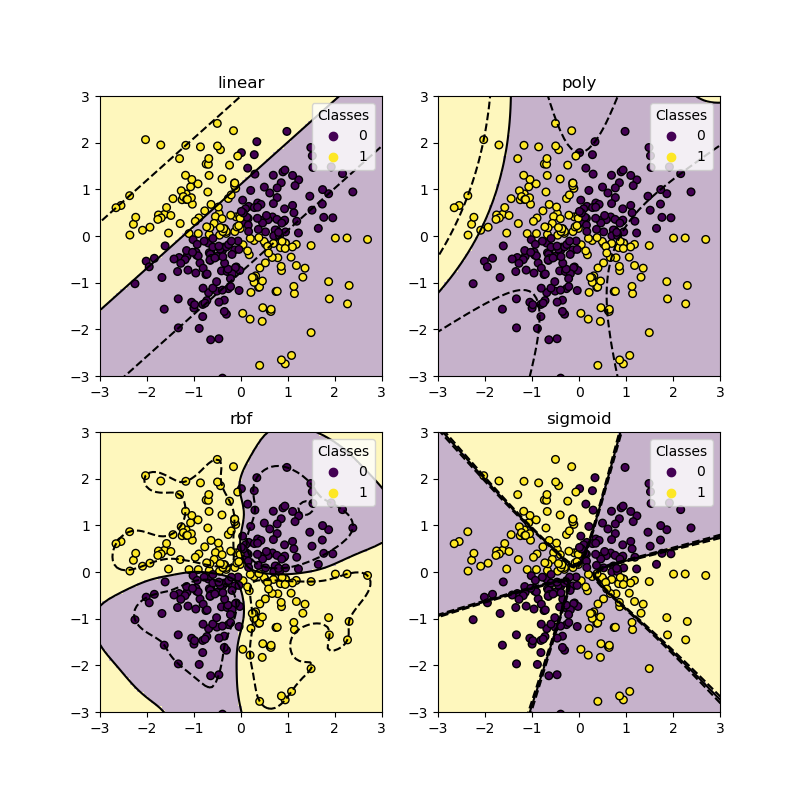
\includegraphics[width=0.6\textwidth]{img/r3/kernels.png}
	\caption{Przykłady granic decyzyjnych w przestrzeni cech na zbiorze XOR\cite{sklearn_api}}
	\label{jadro_svm}
\end{figure}

% \begin{figure}[!htbp]
% 	\centering
% 	\caption{Wykresy wybranych funckji aktywacji}
% 	\begin{subfigure}[b]{0.4\textwidth}
% 		\centering
% 		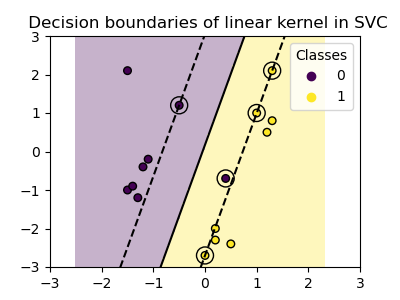
\includegraphics[width=\linewidth]{img/r3/kerlen_linear.png}
% 		\caption{ReLU}
% 		\label{fig:wykres2}
% 	\end{subfigure}
% 	\hfill
% 	\begin{subfigure}[b]{0.4\textwidth}
% 		\centering
% 		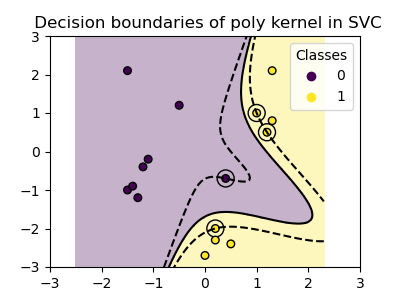
\includegraphics[width=\linewidth]{img/r3/kerlen_poly.png}
% 		\caption{Sigmoid}
% 		\label{Sigmoid}
% 	\end{subfigure}
% 	\begin{subfigure}[b]{0.4\textwidth}
% 		\centering
% 		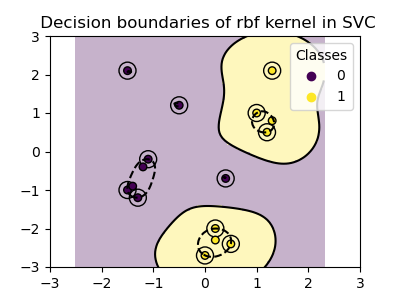
\includegraphics[width=\linewidth]{img/r3/kerlen_rbg.png}
% 		\caption{Sigmoid}
% 		\label{Sigmoid}
% 	\end{subfigure}
% \end{figure}
\newpage
\subsection*{LS-SVM}
LS-SVM stanowi modyfikację klasycznego SVM, w której problem optymalizacji kwadratowej zastąpiono rozwiązaniem układu równań liniowych \cite{suykens2002}. Kluczową różnicą w stosunku do standardowej wersji jest zastosowanie funkcji kosztu w postaci sumy kwadratów błędów oraz wykorzystanie równości jako ograniczeń optymalizacji, zamiast nierówności.

Podejście to znacząco upraszcza obliczenia, czyniąc algorytm bardziej efektywnym pod względem czasu uczenia, szczególnie dla dużych zbiorów danych. Jednakże, uproszczona forma LS-SVM charakteryzuje się większą wrażliwością na obserwacje odstające, co może wpływać na stabilność klasyfikatora w obecności szumu lub nietypowych próbek.

\subsection*{Modele typu Boosting} Koncepcja polegajaca na połaczeniu wielu modeli posiadających małą skuteczność w celu stworzenia jednego modelu o dużej dokładności\cite{valiant1984, kearns1989}. W ogólnym przypadku schemat działania boostingu polega na sekwencyjnym uczeniu modeli, gdzie każdy kolejny model otrzymuje informację o błędach popełnionych przez poprzednie i na tej podstawie stara się poprawić jakość predykcji całego systemu.
\begin{figure}[!h]
	\centering
	\caption{Schemat przetwarznia wstępnego}

	\begin{tikzpicture}
		% Bloki
		\node[draw, align=center, minimum width=2cm, minimum height=1.1cm] (B) at (1.5,0) {Dane \\treningowe};
		\node[draw, align=center, minimum width=2cm, minimum height=1.1cm] (C) at (6,0) {Klasyfikator 1};
		\node[draw, align=center, minimum width=2cm, minimum height=1.1cm] (W_1) at (10,0) {Waga 1};

		\node[draw, align=center, minimum width=2cm, minimum height=1.1cm] (C_P) at (1.5,-2.5) {Ważone\\dane};
		\node[draw, align=center, minimum width=2cm, minimum height=1.1cm] (D) at (6,-2.5) {Klasyfikator 2};
		\node[draw, align=center, minimum width=2cm, minimum height=1.1cm] (W_2) at (10,-2.5) {Waga 2};

		\node[draw, align=center, minimum width=2cm, minimum height=1.1cm] (N) at (1.5,-5.5) {Ważone\\dane};
		\node[draw, align=center, minimum width=2cm, minimum height=1.1cm] (N_P) at (6,-5.5) {Klasyfikator N};

		\node[draw, align=center, minimum width=2cm, minimum height=1.1cm] (wynik) at (13,-2.5) {Łączna\\predykcja};

		\node[draw, align=center, minimum width=2cm, minimum height=1.1cm] (W_N) at (10,-5.5) {Waga N};
		\node at (1.5, -3.75) {\vdots};
		\node at (6, -3.75) {\vdots};
		\node at (10, -3.75) {\vdots};

		% Strzałki
		\draw[->] (B) -- (C) node[midway, above, align=center] {Nauka};
		\draw[->] (C) -- (C_P) node[midway, above, align=center] {};
		\draw[->] (C_P) -- (D) node[midway, above, align=center] {Nauka};
		\draw[->] (N) -- (N_P) node[midway, above, align=center] {Nauka};
		\draw[->] (C) -- (W_1);
		\draw[->] (D) -- (W_2);
		\draw[->] (N_P) -- (W_N);
		\draw[->] (W_1) -- (wynik);
		\draw[->] (W_2) -- (wynik);
		\draw[->] (W_N) -- (wynik);
		\draw[->] (4.8,-4.2) -- (N);
	\end{tikzpicture}
\end{figure}

Największą wadą boostingu jest wysokie ryzyko przeuczenia, wynikające z jego mechanizmu uczenia się na błędach. Takie podejście sprzyja nadmiernemu skupianiu się na przykładach trudnych do sklasyfikowania, co może prowadzić do zbyt mocnego dopasowania modelu do danych treningowych i utraty zdolności generalizacji.

Zdecydowano się na wybór trzech modeli typu boosting, opartych na technice \textit{Gradient Boosting}, czyli metodzie polegającej na sekwencyjnym minimalizowaniu funkcji straty poprzednich modeli przy użyciu algorytmu spadku gradientowego. Wybrane modele:
\begin{itemize}
	\item \textbf{XGBoost} - wykorzystuje modele drzew decyzyjnych, w każdej iteracji dodając kolejne drzewo, które uczy się na podstawie błędów poprzednich. W celu minimalizacji funkcji straty stosowane jest rozwinięcie Taylora drugiego rzędu, a także regularyzacja L1 i L2 w celu zapobiega przeuczeniu.

	\item \textbf{CatBoost} - podobnie jak XGBoost opiera się na drzewach decyzyjnych i metodzie gradient boosting, jednak dodatkowo optymalizuje przetwarzanie cech kategorycznych i zmniejsza ryzyko przeuczania wprowadzajac mechanizm uporządkowane wzmocnienie

	\item \textbf{LightBoost} - również bazuje na drzewach decyzyjnych, jednak w procesie uczenia nie tworzy całych nowych drzew, lecz rozwija istniejące liście tych drzew, które posiadają najwyższą wartość funkcji straty.

\end{itemize}

\section{Sieci neuronowe}
Neuron, będący podstawowym elementem sztucznej sieci neuronowej, jest inspirowany budową i działaniem neuronów biologicznych występujących w ośrodkowym układzie nerwowym. Komórki nerwowe pełnią funkcję przekaźników impulsów elektrycznych - odbierają, przetwarzają i przekazują sygnały.\\

Neuron matematyczny jest układem typu MISO (Multiple Input, Single Output), który sumuje otrzymane sygnały wejściowe po uprzednim przemnożeniu ich przez odpowiadające im wagi. Do takiej zsumowanej wartości dodawany jest składnik stały, zwany biasem. Ostatecznie wynik ten podawany jest na wejście funkcji aktywacji, której celem jest wprowadzenie nieliniowości do modelu\cite{hertz1993}.



\begin{figure}[!ht]
	\centering
	\begin{tikzpicture}[]

		% Neuron (sumator)
		\draw (9,12.75) circle (1.5);
		\node at (9,12.75) {\scalebox{3}{$\sum$}};
		\node at (9,9.25) {$b$};
		\draw[->] (9,10) -- (9,11.25);

		% Funkcja aktywacji
		\draw (13,13.5) rectangle (16,11.75);
		\draw (13.25,13.25) rectangle (15.75,12);
		\node[font=\Large] at (14.5,12.625) {$f$};

		% Strzałki między blokami
		\draw[->] (10.5,12.75) -- (13,12.75);
		\draw[->] (16,12.75) -- (18.5,12.75);
		\node[font=\Large] at (18.8,12.7) {$y$};
		\node at (11.7,13) {$v$};

		% Wejścia x_i
		\draw[->] (6.25,15) -- (7.75,13.75);
		\draw[->] (6.25,13.5) -- (7.5,13);
		\draw[->] (6.25,10) -- (8,11.5);

		\node at (6,15.5) {$x_1$};
		\node at (5.75,13.5) {$x_2$};
		\node at (5.75,9.75) {$x_N$};

		% Wagi
		\node at (7.25,14.5) {$w_1$};
		\node at (7,13.5) {$w_2$};
		\node at (7.25,10.25) {$w_N$};

		% Kropki między wejściami
		\node at (6.75,12) {.};
		\node at (6.75,11.75) {.};
		\node at (6.75,11.5) {.};

	\end{tikzpicture}
	\caption{Model neuronu}
	\label{Qp}
\end{figure}

Sygnał wyjściowy z pojedyńczego neuronu można wyznaczyć za pomocą wzoru:
\begin{equation}
	y = f\left( \sum_{i=1}^{\text{N}} w_i x_i + \text{b} \right),
\end{equation}

gdzie:
\begin{itemize}
	\item $y$ - sygnał wyjściowy,
	\item $f(\cdot)$ - funkcja aktywacji,
	\item N - liczba wejść,
	\item $x_i$ - sygnał wejściowy dla $i$-tego wejścia,
	\item $w_i$ - waga przypisana do $i$-tego sygnału wejściowego,
	\item b - składnik stały,
\end{itemize}


Organizując neurony warstwowo, tworzymy sieć neuronową. Sieć posiada warstwę wejściową, która przyjmuje dane - liczba neuronów w tej warstwie odpowiada liczbie wymiarów danych wejściowych. Kolejne warstwy nazywane są warstwami ukrytymi, ponieważ nie mamy bezpośredniego dostępu do ich wyjść. Ostatnia warstwa to warstwa wyjściowa, w której liczba neuronów odpowiada liczbie klas w problemie klasyfikacji lub liczbie wartości przewidywanych w problemie regresji.\\




\begin{figure}[h!]
	\centering
	\begin{tikzpicture}[
		node distance=0.5cm and 2cm,
		process/.style={draw, rectangle, minimum width=3.5cm, minimum height=1cm, align=center},
		decision/.style={draw, diamond, aspect=2, minimum width=3.5cm, align=center},
		arrow/.style={-{Latex}, thick}
		]

		% Nodes
		\node[process] (start) {Start};
		\node[process] (init) [below=of start] {Inicjalizacja wag};
		\node[process] (forward) [below=of init] {Propagacja w przód};
		\node[process] (loss) [below=of forward] {Obliczenie błędu};
		\node[process] (backward) [below=of loss] {Propagacja wsteczna błędu};
		\node[process] (update) [below=of backward] {Aktualizacja wag};
		\node[decision] (check) [below=of update] {Czy spełniono\\kryterium stopu?};
		\node[process] (end) [below=0.8cm of check] {Stop};

		% Arrows
		\draw[arrow] (start) -- (init);
		\draw[arrow] (init) -- (forward);
		\draw[arrow] (forward) -- (loss);
		\draw[arrow] (loss) -- (backward);
		\draw[arrow] (backward) -- (update);
		\draw[arrow] (update) -- (check);
		\draw[arrow] (check) -- node[right] {tak} (end);

		\draw[thick] (check.west) -- ++(-2,0) coordinate (tmp) node[midway, above] {nie};
		\draw[arrow] (tmp) |- (forward.west);

	\end{tikzpicture}
	\caption{Schemat procesu uczenia sieci neuronowej}
\end{figure}

Nauka sieci neuronowych polega na iteracyjnej aktualizacji wag neuronów w celu minimalizacji funkcji błędu. Proces ten rozpoczyna się od przypisania początkowych wartości wag, które zazwyczaj wybierane są quasi-losowo - jako niewielkie liczby o rozkładzie normalnym. Taki wybór ma na celu zapewnienie różnorodności w początkowym uczeniu się neuronów. Istnieją jednak również bardziej zaawansowane metody inicjalizacji, które uwzględniają właściwości funkcji aktywacji w poszczególnych warstwach sieci.\\
W każdym kroku procesu uczenia dane ze zbioru treningowego są przetwarzane przez sieć neuronową za pomocą algorytmu propagacji w przód. Na podstawie uzyskanych wyników obliczana jest wartość błędu przy użyciu funkcji straty, która określa sposób kwantyfikacji rozbieżności między przewidywaniami modelu a rzeczywistymi wartościami. Następnie wykorzystywany jest optymalizator, który - na podstawie gradientów obliczanych przy pomocy algorytmu propagacji wstecz wyznacza nowe wartości wag neuronów. Ostatecznym etapem jest aktualizacja wag w całej sieci. Proces ten jest powtarzany przez ustaloną liczbę epok lub do momentu spełnienia zdefiniowanego warunku stopu.
\newpage
Wraz z rozwojem sieci neuronowych powstały bardziej złożone sposoby przetwarzania danych. W badaniach wykorzystano następujące typy warstw sieci neuronowych:
\begin{itemize}
	\item Warstwy gęste - klasyczne warstwy w pełni połączone, w których każdy neuron jest połączony z każdym neuronem warstwy kolejnej. Są najczęściej stosowane w prostych sieciach oraz jako warstwy końcowe w bardziej złożonych architekturach.

	\item Warstwy konwolucyjne - przetwarzają dane wejściowe za pomocą filtrów konwolucyjnych, które działają lokalnie w obrębie małych fragmentów danych wejściowych, zgodnie z przesuwającym się jądrem. Podczas procesu uczenia, wartości wag jądra są aktualizowane, co pozwala na automatyczne wykrywanie cech. Często stosowanym mechanizmem pomocniczym jest warstwa poolingowa, której zadaniem jest redukcja wymiarowości danych oraz zwiększenie odporności na przesunięcia i zakłócenia.
	      Zastosowanie warstw konwolucyjnych umożliwiło rozwój głębokiego uczenia, eliminując konieczność ręcznego projektowania wektora cech przez inżynierów.

	\item Warswy LSTM - specjalny typ rekurencyjnych warstw neuronowych zaprojektowany w celu ograniczenia problemu zanikających gradientów, czyli zjawiska, w którym wartości gradientów w początkowych warstwach stają się bardzo małe, co prowadzi do niestabilności i spowolnienia procesu uczenia. Warstwy LSTM wprowadzają pamięć krótkotrwałą, która jest kontrolowana przez trzy rodzaje bramek: wejściową, wyjściową oraz zapominającą. Bramki te regulują przepływ informacji do, z oraz w obrębie komórki pamięci, co umożliwia skuteczne przechowywanie i aktualizowanie informacji w czasie. Dzięki temu model jest w stanie uczyć się zależności sekwencyjnych na dłuższych dystansach czasowych. Choć mechanizm LSTM znacząco ogranicza problem zanikania gradientów, nadal może wystąpić zjawisko eksplodujących gradientów. Warstwy te są szczególnie przydatne podczas przewidywania szeregów czasowych.
\end{itemize}
Tworząc sieć neuronową, inżynier musi dostosować hiperparametry, które determinują zarówno strukturę sieci, jak i sposób jej uczenia. Hiperparametry dzielą się na dwie główne kategorie:
\begin{enumerate}
	\item Hiperparametry związane z architekturą sieci:
	      \begin{enumerate}
		      \item Liczba warstw sieci,
		      \item Liczba neuronów w poszczególnych warstwach,
		      \item Funkcje aktywacji zastosowane w warstwach,
		      \item Typy warstw.
	      \end{enumerate}
	\item Hiperparametry związane z procesem uczenia:
	      \begin{enumerate}
		      \item Liczba epok - warunek stopu związany z ilością prztworzeń zbiorzu uczącego,
		      \item Funkcja strat - miara błędu wykorzystywana przez optymalizator do aktualizacji wag,
		      \item Optymalizator -  algorytm obliczający gradienty, wyznacza nowe wagi podczas procesu nauki.
		      \item Wielkość wsadu - liczba próbek przetwarzanych jednocześnie w jednej iteracji,
		      \item Tempo uczenia - parametr regulujący krok aktualizacji wag.
	      \end{enumerate}
\end{enumerate}

Proces wyboru hiperparametrów jest kluczowy dla uzyskania modelu o wysokiej skuteczności. Wraz ze zwiększaniem liczby warstw sieci oraz liczby neuronów, rośnie zdolność modelu do reprezentowania złożonych zależności, co prowadzi do zmniejszenia błędu biasu. Jednak bardziej złożone modele posiadają większy rozrzut wyników co skutkuje wzrostem wariancji

\begin{figure}[!h]
	\centering
	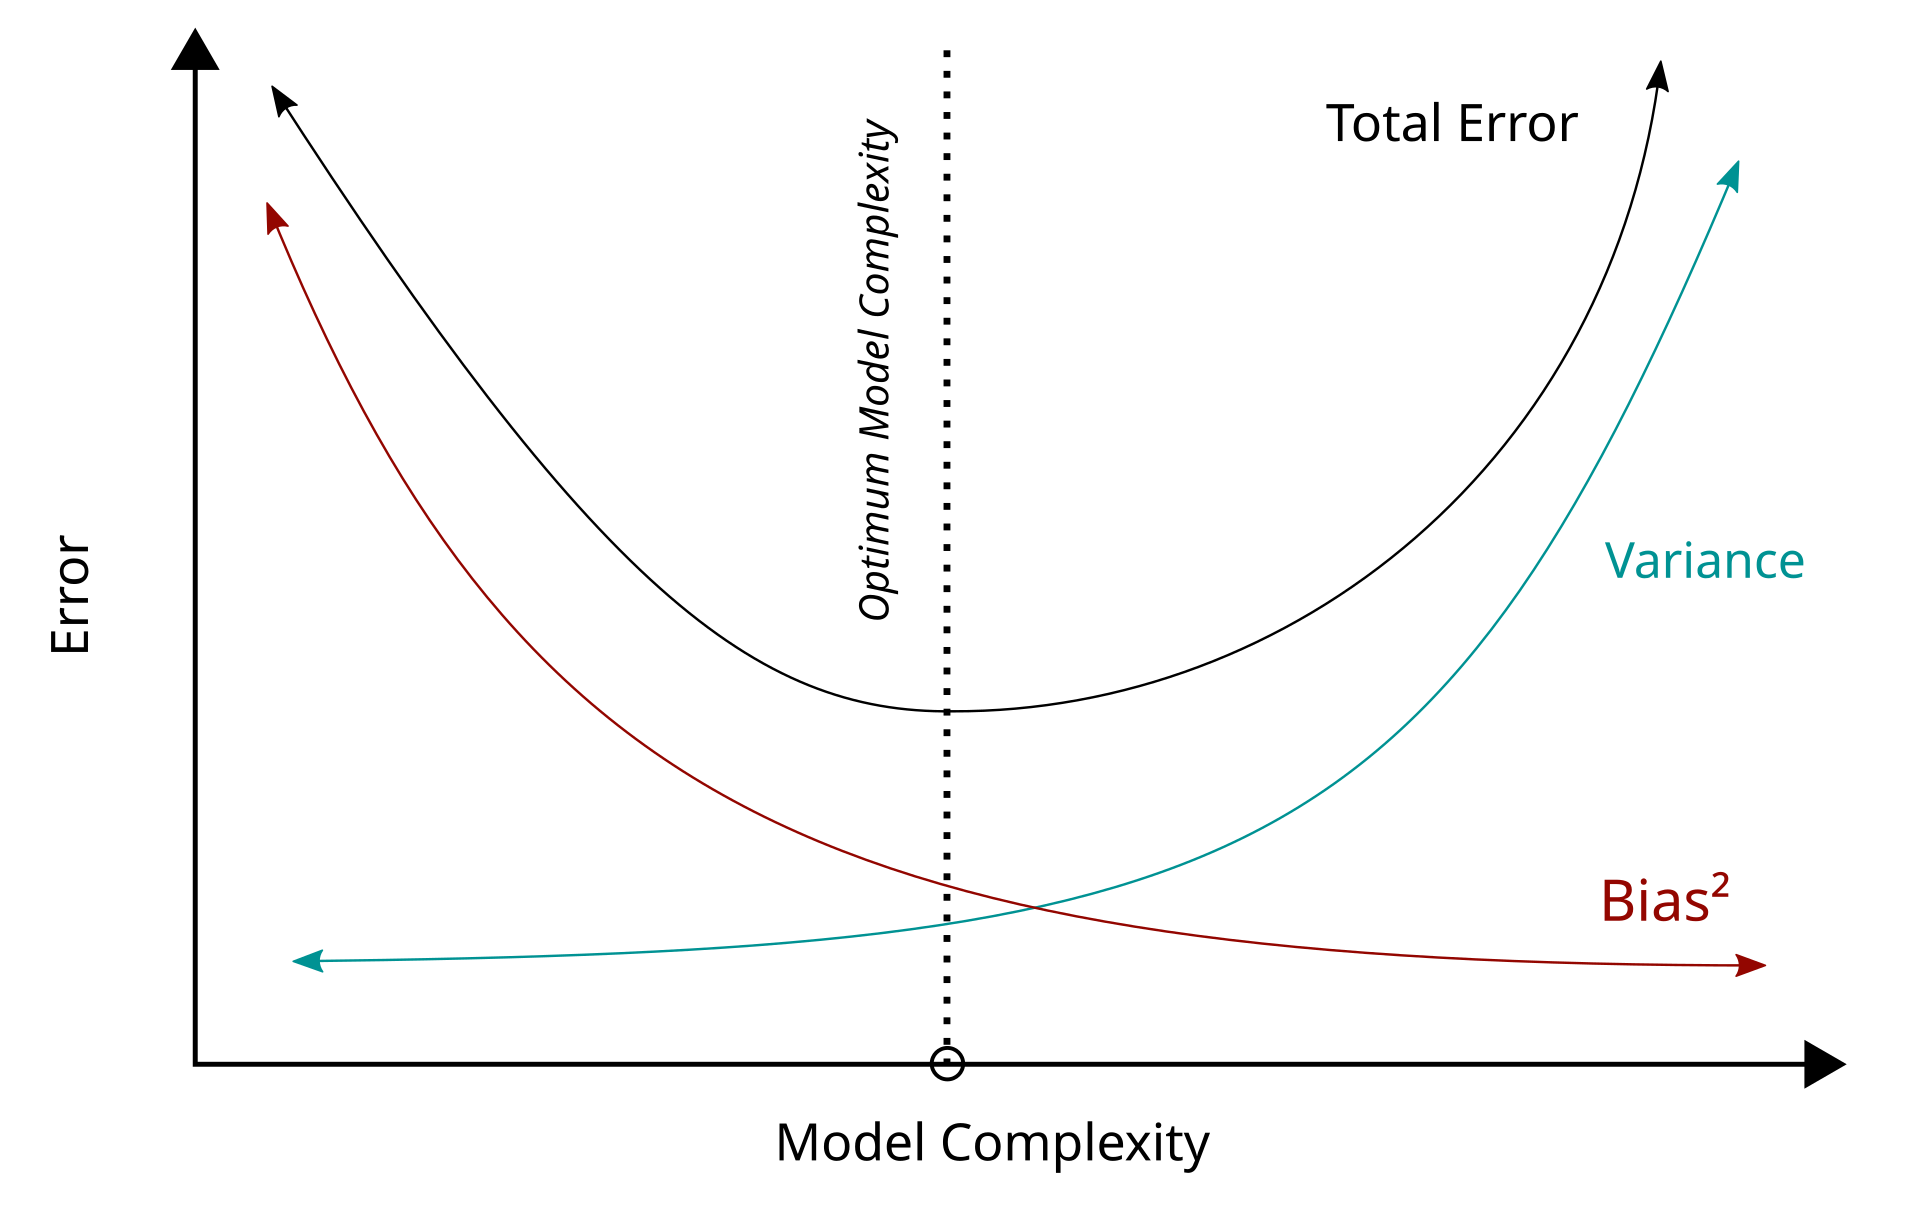
\includegraphics[width=0.8\textwidth]{img/r3/Bias_and_variance_tradeoff.png}
	\caption{Zależność pomiędzy wariancją a biasem w funkcji złożoności modelu\cite{bigbossfarin2021}}
	\label{bias-variance tradeoff}
\end{figure}
\newpage
Wykres przedstawia \ref{bias-variance tradeoff} kompromis obciążeniowo-wariacyjny (bias-variance tradeoff) w funkcji złożoności modelu. Przy niskiej złożoności model nie jest w stanie dobrze odwzorować zależności w zbiorze uczącym - mamy wówczas do czynienia z niedouczeniem oraz wysokim błędem obciążenia. Wraz ze wzrostem złożoności modelu błąd obciążenia maleje, a jakość predykcji rośnie. Jednak dalsze zwiększanie złożoności prowadzi do wzrostu błędu wariancji, ponieważ model zaczyna uczyć się również szumu obecnego w danych, co skutkuje przeuczeniem i utratą zdolności generalizacji. W takiej sytuacji mimo niskiego błędu obciążenia, wysoka wariancja obniża skuteczność modelu. Optymalny punkt znajduje się tam, gdzie suma błędu obciążenia i wariancji jest najmniejsza - w tym miejscu model osiąga najlepszą równowagę między niedouczeniem a przeuczeniem.


\section{Miary jakościowe klasyfikatorów}
W celu efektywnego porównywania modeli predykcyjnych konieczne jest zastosowanie odpowiednich miar oceny jakości, które umożliwiają liczbową ocenę skuteczności działania danego modelu w określonym kontekście. Dobór metryk powinien być dostosowany do charakteru problemu - inne miary stosuje się w przypadku klasyfikacji, inne przy lokalizacji obiektów, a jeszcze inne przy zadaniach regresyjnych.\\

Aby właściwie zrozumieć sposób działania metryk stosowanych w klasyfikacji binarnej, należy w pierwszej kolejności zdefiniować cztery możliwe wyniki predykcji:
\begin{itemize}
	\item \textbf{True Positive (TP)} - poprawna klasyfikacja przypadku z arytmią serca jako przypadek chorobowy.
	\item \textbf{False Positive (FP)} - błędna klasyfikacja przypadku zdrowego jako przypadek z arytmią. Nazywana również błędem pierwszego rodzaju.
	\item \textbf{True Negative (TN)} - poprawna klasyfikacja przypadku zdrowego jako niechorobowego.
	\item \textbf{False Negative (FN)} - błędna klasyfikacja przypadku z arytmią jako przypadek zdrowy. Nazywana również błędem drugiego rodzaju.
\end{itemize}
Dzięki wyznaczeniu 4 przypadów, jestesmy w stanie w graficzny sposób przedstawić wyniki klasyfikacji w postaci macierzy pomyłek.

\begin{figure}[!h]
	\centering
	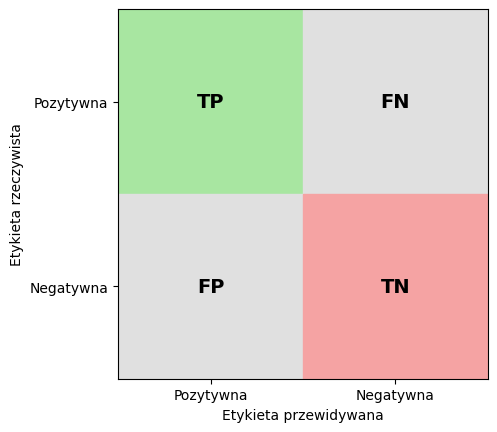
\includegraphics[width=0.5\textwidth]{img/r3/error_matrix.png}
	\caption{Struktura macierzy pomyłek dla klasyfikacji binarnej}
	\label{fig:etykieta-rysunku}
\end{figure}

Wykorzystując wymieniane przypadki, jesteśmy w stanie wyznaczyć metryki jakościowe, które pozwalają na ocenę skuteczności klasyfikatora.

\begin{itemize}
	\item \textbf{Dokładność} - metryka określająca jaki procent przypadków został poprawnie sklasyfikowany. Jest to metryka która jest mocno zalezna od rozkładu klasy. W sytuacji gdy jedna klasas jest znacznie liczniejsza, może ona mocno zakrzywić wyniki. W przypadku klasyfykacji binarnej możemy ją wyznaczyć jako:
	      \begin{equation}
		      \text{Accuracy} = \frac{\text{TP + TN}}{\text{TP + FP + TN + FN}}
	      \end{equation}

	\item \textbf{Precyzja} - miara jakościowa określającą jaki procent przypadków sklasyfikowanych jako osoby z chorobą rzeczywiscie posiadaja arytmię. Prezycja nie zwraca uwagi na przypadki zdrowę, zwraca uwagę jedynie na przypadki z arytmią. Omawianą miarę możemy obliczyć jako:
	      \begin{equation}
		      \text{Precision} = \frac{\text{TP}}{\text{TP + FP}}
	      \end{equation}

	\item \textbf{Swoistość} - określa umiejętność detekcji zdrowych pacejntów bez arytmi. Matematycznie możemy zapisać to jako:

	      \begin{equation}
		      \text{Specificity} = \frac{\text{TN}}{\text{TN + FP}}
	      \end{equation}
	\item \textbf{Czułość} - prawdopodobieństwo ze klasyfikacja będzie poprawna pod warunkiem że dana próbka pochodzi od osoby chorej. Można ją obliczyć ze wzoru:

	      \begin{equation}
		      \text{Recall} = \frac{\text{TP}}{\text{TP + FN}}
	      \end{equation}


	\item \textbf{F-miara} - metryka która łaczy prezycję i czułosć. Wyznacza się jako średnią harmoniczną owych metryk. Ze względu na to, jest ona bardzo wrażliwa na przypadki gdy jedna z metryk jest bardzo niska. Jednak jest ona odporna na nierówny rozkład klas. Wartość F-miary możemy wyznaczyć jako:

	      \begin{equation}
		      \text{F}_1 = \frac{1}{2} \left( \frac{1}{\text{precision}} + \frac{1}{\text{recall}} \right) = \frac{2 \cdot \text{precision} \cdot \text{recall}}{\text{precision} + \text{recall}} = \frac{\text{2TP}}{\text{2TP + FP + FN}}
	      \end{equation}


	\item \textbf{współczynnika korelacji Matthews'a (MCC)} - miara korelacji binarnej wprowadzona do uczenia maszynowego przez Briana W. Matthewsa~\cite{matthews1975}. Zakres tego współczynnika wynosi od $-1$ do $1$, gdzie $1$ oznacza perfekcyjną klasyfikację, $0$ klasyfikację losową, a $-1$ - całkowicie odwrotną predykcję. MCC jest wskaźnikiem jakościowym odpornym na niezbalansowanie klas i można go obliczyć według wzoru:

	      \begin{equation}
		      \text{MCC} = \frac{\text{TP} \cdot \text{TN} - \text{FP} \cdot \text{FN}}{\sqrt{(\text{TP} + \text{FP})(\text{TP} + \text{FN})(\text{TN} + \text{FP})(\text{TN} + \text{FN})}}
	      \end{equation}

	\item \textbf{Krzywa ROC} \cite{altman1994, brown2006roc, fawcett2006} - graficzne przedstawienie wydajności modelu klasyfikacyjnego w zadaniu klasyfikacji binarnej, w zależności od wartości progu decyzyjnego. Wykres ten ukazuje zależność między czułością a 1 - swoistością.

	      \begin{figure}[!h]
		      \centering
		      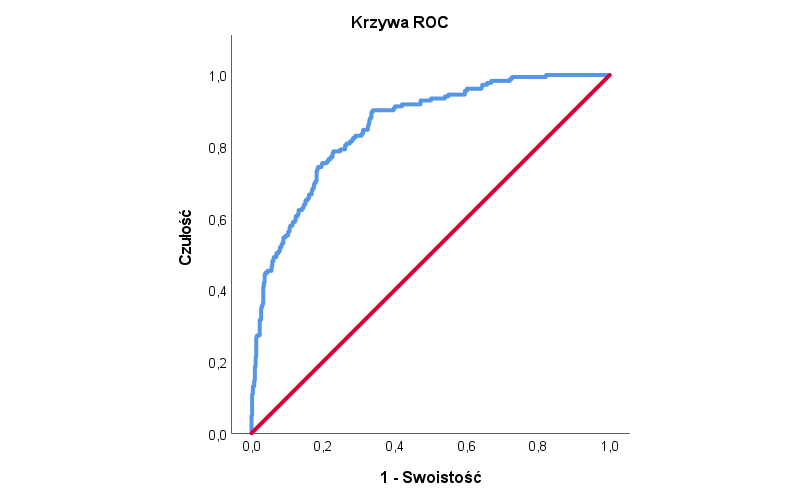
\includegraphics[width=1\textwidth]{img/r4/Krzywa_ROC.png}
		      \caption{Wykres krzywej ROC \cite{solecki2025roc}}
		      \label{fig:etykieta-rysunku}
	      \end{figure}

	      Krzywa ROC służy do oceny oraz porównywania jakości klasyfikatorów, a także do wyboru odpowiedniego progu decyzyjnego, od którego próbki są przypisywane do klasy pozytywnej.

	      W najlepszym przypadku krzywa ROC przechodzi przez punkt (0,0) i (0,1), co oznacza, że klasyfikator osiąga 100\% czułości (brak fałszywie negatywnych wyników) oraz 100\% swoistości (brak fałszywie pozytywnych wyników). Taki model zawsze dokonuje poprawnych predykcji i uznawany jest za idealny.
	      \newpage
	      Wraz z pogorszeniem jakości klasyfikatora krzywa ROC zbliża się do przekątnej łączącej punkty (0,0) i (1,1). Taka linia reprezentuje model losowy - jego predykcje są statystycznie równoważne zgadywaniu, niezależnie od przyjętego progu decyzyjnego. W takiej sytuacji model uznaje się za nieskuteczny.

	      W skrajnie niekorzystnym przypadku, gdy krzywa ROC znajduje się poniżej tej przekątnej, oznacza to, że klasyfikator częściej się myli, niż przewiduje poprawnie. Paradoksalnie, odwrócenie jego predykcj poprawia skuteczność klasyfikacji.

	      Wraz ze zmniejszaniem wartości progu decyzyjnego rośnie czułość modelu, co oznacza spadek liczby błędów drugiego rodzaju. Jednocześnie jednak rośnie liczba błędów pierwszego rodzaju - fałszywie pozytywnych wyników. Z kolei zwiększanie progu skutkuje sytuacją odwrotną: poprawia się swoistość, ale kosztem spadku czułości.

	      Taką sytuacje określa się jako kompromis między czułością a swoistością. Optymalny próg zależy od charakterystyki problemu oraz kosztów błędnych decyzji. W zastosowaniach medycznych często preferuje się modele o wysokiej czułości, aby ograniczyć liczbę niewykrytych przypadków choroby, nawet kosztem większej liczby fałszywych alarmów.

	      Wykorzystując krzywą ROC, możliwe jest oblicznie pod nią. Taka matryka nazywa się \textbf{AUC}. Jest ona zależna i od czułości i od swoistości, wiec jest nie ma nią wpływu niezbalansowanie klas. Jednak,  AUC może prowadzić do mylących wniosków w przypadku przecinających się krzywych ROC, gdzie jednej model może być lepsza w jednym zakresie wartości progu decyzyjnego, a gorsza w innym. W takich sytuacjach wykorzystuje się analizę fragmentaryczną\cite{mcclish1989roc}


	\item \textbf{Funkcja celu (FC)} - w celu ułatwienia porównań pomiędzy różnymi modelami klasyfikacyjnymi zaproponowano autorską metrykę, będącą średnią ważoną trzech niezależnych miar jakości klasyfikacji: swoistości, F-miary oraz współczynnika korelacji Matthews'a (MCC).

	      Ze względu na odmienny zakres wartości MCC (\mbox{-1} do 1), dokonano jego normalizacji do przedziału [0,1] według wzoru:
	      \begin{equation}
		      \text{nMCC} = \frac{\text{MCC} + 1}{2}
	      \end{equation}
	      Zaproponowano następujące wagi: 0.5 dla F-miary, 0.3 dla swoistości oraz 0.2 dla znormalizowanego MCC. Wszystkie składowe funkcji celu przyjmują wartości z zakresu [0,1], co zapewnia ich porównywalność oraz umożliwia interpretację FC jako skali ogólnej jakości klasyfikatora.

	      Funkcję celu definiuje wzór:
	      \begin{equation}
		      \text{FC} = 0.5 \cdot F_1 + 0.3 \cdot \text{Spec} +  0.2 \cdot \text{nMCC}
	      \end{equation}

	      Opisana funkcja celu, zostanie także wykorzystana jako parametr optymalizacji hiperparametrów, który będzie maksymalizowano podczas eksperymentów.

\end{itemize}















\chapter{Przetwarzanie i wybrane zbiory danych}
\section{Przegląd wykorzystanych zbiorów danych}
TODO - napisać coś tutaj
\subsection{MIMIC PERform AF Dataset}
Zbiór danych MIMIC PERform AF\cite{mimic_perform_af} został pozyskany z bazy MIMIC-III Waveform Database Matched Subset\cite{mimiciii_waveform_matched}. Zawiera on 20-minutowe zapisy sygnałów fotopletyzmograficznych oraz elektrokardiograficznych, zarejestrowane u 35 ciężko chorych dorosłych pacjentów hospitalizowanych na oddziałach intensywnej terapii. U 19 z tych pacjentów zdiagnozowano migotanie przedsionków, natomiast u pozostałych zapis sygnałów nie wykazywał nieprawidłowości w rytmie serca. Dane zostały zebrane z wykorzystaniem monitora przyłóżkowego, z częstotliwością próbkowania wynoszącą 125 Hz.

\subsection{Zbiór PPG według Liu, Zengding i Zhou et al.}
Dane wykorzystywane w tym zbiorze\cite{liu2022multiclass} zostały zebrane w okresie od marca 2020 do marca 2021 w szpitalu Fuwai w Pekinie, będącym wyspecjalizowaną placówką w zakresie chorób sercowo-naczyniowych. Sygnał fotopletyzmograficzny został początkowo próbkowany z częstotliwością 250 Hz, a następnie poddany procesowi resamplingu do 100 Hz. W celu usunięcia niepożądanych zakłóceń zastosowano filtrację pasmową w zakresie 0.5 - 50 Hz. Przefiltrowany sygnał został następnie podzielony na segmenty 10-sekundowe, przy czym fragmenty zawierające istotne zakłócenia zostały odrzucone.


Cały zbiór danych obejmuje zapisy od 228 pacjentów, co odpowiada łącznie 118 217 segmentom 10-sekundowym. Na potrzeby badań publicznych udostępniono jedynie 46 827 z tych fragmentów. Dane zostały skategoryzowane według pięciu typów arytmii: przedwczesny skurcz komorowy, przedwczesny skurcz przedsionkowy, tachykardia komorowa, tachykardia nadkomorowa oraz migotanie przedsionków.

\subsection{PhysioNet/CinC Challenge 2015}
test\cite{physionet_challenge_2015} Jest zbiorem użytym w konkursie majacym na celu stworzenie algorytmu redukującego ilość fałszych alarmów podczas detekcji arytmii serca. Dane pochodzą z czterech losowo wybranch, szpitali w Stanach Zjednoczonych oraz Europie. Udostępniona część zbioru zawiera 750 nagrań. Sygnały zostały próbkowane z częstotliwością 250Hz oraz przefiltrowane filtrem pasmowym 0.05 - 40Hz
\subsection{Dane syntetyczne}
W celu wzbogacenia zbiorów danych, zdecydowano użyć się danych syntetycznych wygenerowanych przy użyciu generatora sygnałów PPG i ECG z epizodami arrytmi\cite{solosenko2022}. Zastosowany symulator umożliwia pełną kontrolę nad procesem generowania sygnałów. Użytkownik ma możliwość definiowania szeregu parametrów determinujących charakterystykę sygnału, w tym: rodzaj arrytmi, mediane dłguości epizodów arytmi, obciążenie arytmią które determinuje łączny czas kiedy występuje arytmia, wskaźnik przedwczesnychskurczów przedsionkowych czy rodzaj pulsu zdefiniowany przez Dawber et al\cite{dawber1973dicrotic}.
\begin{figure}[!h]
	\centering
	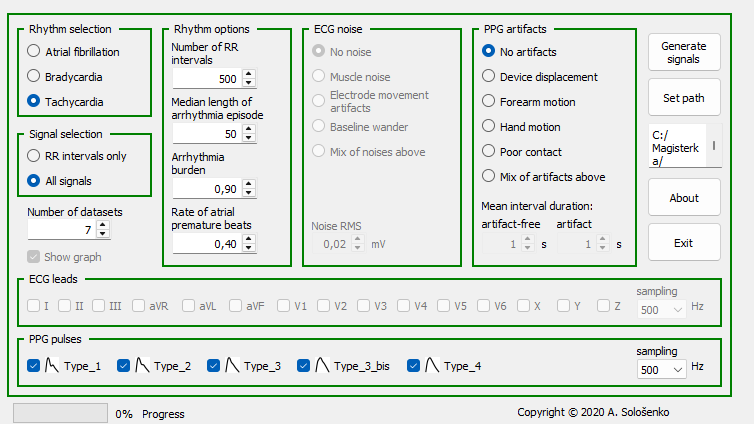
\includegraphics[width=1\textwidth]{img/r4/symulator_GUI.png}
	\caption{GUI użytego symulatora}
	\label{fig:etykieta-rysunku}
\end{figure}\\

W ramach eksperymentu wygenerowano pięć syntetycznych podzbiorów danych, z których każdy został zasymulowany z częstotliwością próbkowania równą 500 Hz oraz zawierał sygnały odpowiadające 500 kolejnym interwałom RR. Każdy ze zbiorów zawierał równą ilośc przypadków bradycardii, tachycardii i migotania przedsionków. Zawierał się w nich także każdy rodzaj pulsu PPG. Zdecydowano się nie wykorzystywać możliwości generowania sygnałów z szumem.

Poszczególne podzbiory różniły się parametrami charakterystycznymi dla przebiegu arytmii:

\begin{table}[ht]
	\centering
	\caption{Porównanie parametrów podzbiorów danych syntetycznych}
	\begin{tabular}{
			@{}c
			S[table-format=2.0]
			S[table-format=1.1]
			S[table-format=1.2]
			@{}
		}
		\toprule
		Zbiór &
		\multicolumn{1}{c}{\makecell{Mediana długości        \\ epizodu arytmii}} &
		\multicolumn{1}{c}{\makecell{Obciążenie              \\ arytmią}} &
		\multicolumn{1}{c}{\makecell{Wskaźnik przedwczesnych \\ skurczów przedsionkowych}} \\
		\midrule
		1     & 3  & 0.1 & 0.05                              \\
		2     & 10 & 0.3 & 0.10                              \\
		3     & 5  & 0.5 & 0.10                              \\
		4     & 30 & 0.4 & 0.20                              \\
		5     & 50 & 0.9 & 0.40                              \\
		\bottomrule
	\end{tabular}
\end{table}

Każdy ze zbiorów ma symulować inny rodzaj arytmi:
\begin{itemize}
	\item Zbiór 1 - Rzadkie występowanie krótkich epizodów arytmi
	\item Zbiór 2 - Umiarkowane występowanie z umiarkowaną liczbą przedwczesnych skórczy
	\item Zbiór 3 - Wysokie występowanie arytmi z krótkimi epizodami
	\item Zbiór 4 - Długie, częste epizody arytmi.
	\item Zbiór 5 - Niemal ciągła arytmia
\end{itemize}

Dzięki zastosowanemu symulatorowi, wygenerowane dane syntetyczne mogą stanowić cenne źródło informacji dla przyszłych modeli klasyfikacyjnych. Umożliwiają one nie tylko lepsze zrozumienie przypadków odstających, ale również wspierają proces uczenia modeli w scenariuszach bardziej typowych, odpowiadających klasycznym przypadkom klinicznym.

\section{Przetwarzanie wstępne}
Pomimo wysokiej jakości wybranych zbiorów danych, ich bezpośrednie wykorzystanie w procesie klasyfikacji wymaga zastosowania wieloetapowego przetwarzania wstępnego. Głównym celem tych transformacji jest ujednolicenie charakterystyki sygnałów pochodzących z różnych źródeł oraz przygotowanie reprezentatywnego wektora cech, który może zostać wykorzystany w procesie uczenia klasyfikatorów.\\

\newpage
Pierwszym etapem przetwarzania wstępnego sygnału jest jego filtracja. W tym celu zastosowano filtr pasmowo-przepustowy o częstotliwościach granicznych 0.5 Hz oraz 40 Hz. Głównym celem tak dobranego filtra jest eliminacja zakłóceń pochodzących spoza pasma istotnego z punktu widzenia analizy sygnałów PPG. Dolne ograniczenie pozwala zmniejszyć wpływ ruchu pacjenta czy zmiane położenia czujnika, natomiast górna granica redukuje wpływ wysokoczęstotliwościowych zakłóceń, takich jak zakłócenia elektromagnetyczne.\\

Drugim istotnym etapem przetwarzania wstępnego była zmiana częstotliwości próbkowania sygnałów. Zdecydowano się na jednolitą częstotliwość 100 Hz, co odpowiada najniższej wartości występującej wśród wykorzystanych zbiorów danych. Ujednolicenie próbkowania do tej wartości niesie ze sobą kilka korzyści. Po pierwsze, redukcja liczby próbek skutkuje zmniejszeniem rozmiaru danych, co przekłada się na krótszy czas ich przetwarzania jak i nauki modeli w sposób bezcechowych.\\

Kolejnym krokiem w procesie przetwarzania wstępnego była normalizacja sygnału do przedziału $[0, 1]$. Wykorzystane zbiory danych charakteryzowały się zróżnicowanym zakresem wartości amplitud, co mogłoby negatywnie wpłynąć zarówno na proces uczenia cechowego, jak i bezcechowego. Niejednorodna skala danych może prowadzić do dominacji niektórych sygnałów lub cech w trakcie uczenia. W celu minimalizacji tego efektu, zdecydowano się na niezależną normalizację każdego sygnału osobno.\\

Z uwagi na fakt, że zbiór danych opracowany przez Liu, Zengding i Zhou et al.\cite{liu2022multiclass} składa się z 10-sekundowych segmentów sygnału, zdecydowano o ujednoliceniu długości wszystkich pozostałych próbek poprzez ich podział na fragmenty o identycznym czasie trwania. Segmentacja została przeprowadzona po wcześniejszym przeskalowaniu częstotliwości próbkowania do 100 Hz, co oznacza, że każdy 10-sekundowy segment zawiera dokładnie 1000 próbek. Próbki te, zostaną wykorzytane do bezcechowej nauki klasyfikatorów.\\

Ostatnim etapem przetwarznia wstępnego jest wybranie oraz ekstrakcja cech. Proces ten zostanie omówiony dokładnie w rozdziale \ref{Ekstrakcja cech}

\begin{figure}[!h]
	\caption{Schemat przetwarznia wstępnego}

	\begin{tikzpicture}
		% Bloki
		\node[draw, align=center, minimum width=2cm, minimum height=1.1cm] (B) at (0.5,0) {Filtr\\pasmowy};
		\node[draw, align=center, minimum width=2cm, minimum height=1.1cm] (C) at (3.05,0) {Resampler};
		\node[draw, align=center, minimum width=2cm, minimum height=1.1cm] (D) at (5.9,0) {Normalizator};
		\node[draw, align=center, minimum width=2cm, minimum height=1.1cm] (E) at (8.9,0) {Segmentator};
		\node[draw, align=center, minimum width=2cm, minimum height=1.1cm] (F) at (11.7,0) {Ekstraktor\\cech};

		% Strzałki
		\draw[->] (-2,0) -- (B.west)
		node[midway, above, align=center] {Bazowy\\sygnał};
		\draw[->] (B) -- (C) node[midway] {};
		\draw[->] (C) -- (D) node[midway] {};
		\draw[->] (D) -- (E) node[midway] {};
		\draw[->] (E) -- (F.west) node[midway] {};
		\draw[->] (F.east) -- (14,0)
		node[midway, above, align=center]{Wektor\\cech};
		\draw[-] (E.east) -- (11,-2.5)
		node[midway, above, align=center]{};
		\draw[->] (11,-2.5) -- (14,-2.5)
		node[midway, above, align=center]{Segmentowany\\sygnał};

	\end{tikzpicture}
\end{figure}

\newpage
\section{Ekstrakcja cech}
\label{Ekstrakcja cech}
Zdecydowano się na wybór czterech głównych domen analizy, z których każda interpretuje sygnał PPG z innej perspektywy, umożliwiając wydobycie zróżnicowanych informacji. Niezależnie od wybranej domeny, we wszystkich przypadkach zastosowano zestaw podstawowych miar statystycznych, które zostały wyekstrahowane z przekształconych sygnałów:
\begin{itemize}
	\item Średnia arytmetyczna,
	\item Mediana,
	\item Odchylenie standardowe,
	\item Wariancja,
	\item Rozstęp międzykwartylowy,
\end{itemize}

\subsection{Cechy z domeny czasu}
Pierwszą z wybranych domen, interpretuje sygnał jako funkcję ciągłą w czasie. Domena czasu trakuje kolejne próbki czasowe jako kolejne wartości funkcji aplitudy. Domena ta bezpośrednio analizuje sygnału w jej pierwotnej postaci, gdzie $x = \{x_1, x_2, \ldots, x_n\}$. W tej przestrzeni, zdecydowano się na wybranie następujących cech:
\begin{itemize}
	\item \textbf{Skośność} - miara asymetrii sygnału:
	      \begin{equation}
		      \frac{1}{N} \sum_{i=1}^{N} \left( \frac{x_i - \bar{x}}{\sigma} \right)^3
	      \end{equation}
	      gdzie:
	      \begin{itemize}
		      \item \( \bar{x} \) - średnia arytmetyczna.
		      \item \( \sigma \) - odchylenie standardowe sygnału.
	      \end{itemize}
	\item \textbf{Współczynnik zmienności} -  względna miara zróżnicowania sygnału:
	      \begin{equation}
		      \text{CV} = \frac{\sigma}{\bar{x}}
	      \end{equation}
	\item \textbf{Średnie odchylenie bezwzględne} - bezwzgledna miara zróżnicowania sygnału:
	      \begin{equation}
		      \text{MAD} = \frac{1}{n} \sum_{i=1}^{n} \left| x_i - \bar{x} \right|
	      \end{equation}

	\item \textbf{Entropia Shannona} - miara niepewności sygnału:
	      \begin{equation}
		      H = -\sum_{i=1}^{N} p_i \mathrm{log}_{2} p_i
	      \end{equation}
	      gdzie:
	      \begin{itemize}
		      \item \( p_i \) - prawdopodobieństwo wystąpienia \( i \)-tej wartości sygnału.
	      \end{itemize}





\end{itemize}


\subsection{Cechy różnicowe}
Kolejną z wybranych domen jest domena cech różnicowych, w której sygnał nie jest bezpośrednio intereptowany jako kolejne wartości amplitudy, tylko poprzez różnice zmian między kolejnymi próbkami $\Delta x = \{x_2 - x_1,\, x_3 - x_2,\, \ldots,\, x_n - x_{n-1}\}$. Cechy wyekstrachowane z tej domeny:
\begin{itemize}
	\setcounter{enumi}{4}
	\item \textbf{Procent dodatnich różnic} - odsetek dodatkich róznic kolejnych wartości sygnału

	      \begin{equation}
		      \frac{100}{N-1} \sum_{i=1}^{N-1} \delta(\Delta x > 0)
	      \end{equation}
	      gdzie:
	      \begin{itemize}
		      \item \( \delta(\cdot) \) - funkcja wskaźnikowa, równa 1 gdy warunek jest spełniony, 0 w przeciwnym wypadku.
	      \end{itemize}
	\item \textbf{Średnia wartość bezwzględna różnic:}
	      \begin{equation}
		      \frac{1}{N-1} \sum_{i=1}^{N-1} |\Delta x|
	      \end{equation}

	\item \textbf{Pierwiastek średniokwadratowy różnic} - miara zmienności rytmu serca, która odzwierciedla aktywność układu przywspółczulnego:\cite{Farokhipour2023}
	      \begin{equation}
		      \text{RMSSD} = \sqrt{ \frac{1}{N-1} \sum_{i=1}^{N-1} (\Delta x)^2 }
	      \end{equation}

	\item \textbf{Znormalizowane średnie odchylenie bezwzględne różnic} - ocenia lokalną dynamikę zmian sygnału:
	      \begin{equation}
		      \frac{1}{N-1} \sum_{i=1}^{N-1} \frac{|\Delta x|}{\bar{x}}
	      \end{equation}

	\item \textbf{Znormalizowana suma bezwzględnych różnic:}

	      \begin{equation}
		      \frac{\sum_{i=1}^{N-1} |\Delta x|}{\sum_{i=1}^{N} |x_i|}
	      \end{equation}

\end{itemize}


\subsection{Cechy częstotliwościowe}
Ostatnią wybraną domeną jest domena częstotliwościowa. W tej domenie, sygnał jest przekszłcany przy użyciu transoframty Fouriera, aby uzyskać jego rozkład mocny w zależności częstotliwości $P_{xx}(f)$, gdzie $f$ oznacza częstotliwość. Analiza cech częstotliwościowych, pozwala identyfikować składowe dominujące jak i nieregularności. W tej domenie zdecydowano się na ekstrakcję następujących cech:
\begin{itemize}
	\setcounter{enumi}{9}
	\item \textbf{Maksymalny szczyt widmowy} - określa częstotliwość która posiada największą ilość energii
	      \begin{equation}
		      f_{\max} = f \bigl( \arg\max_{f} P_{xx}(f) \bigr)
	      \end{equation}


	\item \textbf{Kurtoza widma} - spłaszczenie widma sygnału:
	      \begin{equation}
		      \text{kurt}(P_{xx}) = \frac{1}{M} \sum_{i=1}^M \left( \frac{P_{xx}(f_i) - \overline{P_{xx}}}{\sigma_{P_{xx}}} \right)^4
	      \end{equation}

	\item \textbf{Energia spektralna} - suma mocy sygnału w całym paśmie częstotliwości:
	      \begin{equation}
		      E = \sum_{i=1}^{M} P_{xx}(f_i)
	      \end{equation}

	\item \textbf{Udział wysokich szczytów widma}
	      \begin{equation}
		      \frac{\sum_{i=1}^{M} \delta(P_{xx}(f_i) > \overline{P_{xx}} )}{M}
	      \end{equation}
\end{itemize}

\subsection{Implementacja}
Wstępne przetwarzanie zbiorów danych zostało zrealizowane z wykorzystaniem środowiska MATLAB w wersji R2024b. Wybór ten podyktowany był faktem, iż większość analizowanych zbiorów danych dostarczana była w postaci plików z rozszerzeniem .mat, będących binarnym formatem przechowywania danych specyficznym dla środowiska MATLAB.\\

Proces wstępnego przekształcania wymagał indywidualnego dostosowania skryptów dla każdego zbioru danych, co wynikało z różnic w sposobie reprezentacji danych. W części przypadków dane zapisane były jako pojedyncze sygnały, natomiast w innych przyjmowały postać struktur zawierających dodatkowe informacje kontekstowe, takie jak metadane dotyczące sygnału oraz dane pacjenta.

Proces zmiany częstotliwości próbkowania sygnału został zrealizowany przy użyciu funkcji \texttt{resample()}. Funkcja ta najpierw przeprowadza interpolację sygnału, zwiększając jego częstotliwość próbkowania, następnie sygnał jest filtrowany za pomocą dolnoprzepustowego filtra FIR, a ostatecznie następuje redukcja częstotliwości próbkowania do wartości docelowej \cite{mathworks_resample_2025}.\\


Proces wyodrębniania wektora cech został również przeprowadzony w środowisku MATLAB. Do obliczenia podstawowych miar statystycznych wykorzystano funkcje dostępne w standardowym pakiecie języka. W przypadku bardziej złożonych cech zastosowano narzędzia udostępniane w ramach rozszerzeń Statistics and Machine Learning Toolbox oraz Signal Processing Toolbox.


\chapter{Detekcja arytmii serca}
Całość skryptów dotyczących detekcji arytmii serca z wykorzystaniem metod uczenia maszynowego została zaimplementowana w języku Python w wersji 3.11. W celu ułatwienia procesu budowy, trenowania oraz ewaluacji klasyfikatorów tradycyjnych wykorzystano bibliotekę scikit-learn, która oferuje szeroki zestaw gotowych algorytmów klasyfikacyjnych, funkcji oceny jakości modeli oraz narzędzi do przetwarzania i transformacji danych. W przypadku implementacji modeli opartych na sztucznych sieciach neuronowych zastosowano bibliotekę TensorFlow.\\

Cały proces nauki i testowania modeli został przeprowadzony na komputerze osobistym o następującej specyfikacji sprzętowej: procesor Intel Core i5-13400F, 32 GB pamięci RAM oraz karta graficzna NVIDIA GeForce RTX 4070.
\section{Architektura i konfiguracja modeli}
W pierwszym etapie nauki zdecydowano się na jedynie nieznaczną modyfikację domyślnych parametrów klasycznych klasyfikatorów. Dla algorytmu K najbliższych sąsiadów zastosowano metrykę Minkowskiego z parametrem q=2, co odpowiada wykorzystaniu klasycznej metryki euklidesowej. Liczbę sąsiadów ustalono na k=50. W przypadku drzewa decyzyjnego ograniczono maksymalną głębokość drzewa do 30 testów logicznych, co miało na celu redukcję ryzyka przeuczenia modelu. Dla klasyfikatora typu las losowy wykorzystano 100 drzew decyzyjnych, z których każde ograniczono do maksymalnie 10 testów logicznych.

Naiwny klasyfikator Bayesa, ze względu na swoje czysto statystyczne działanie, nie posiada klasycznych hiperparametrów wpływających na proces uczenia. Jedynym parametrem regulacyjnym jest wartość wariancji dodawanej do wszystkich cech w celu stabilizacji obliczeń numerycznych, którą ustawiono na $10^{-8}$.
Dopierajac hiperparametry dla metody wektorów nośnych, wybrano jądro rbf które w celu obliczenia odległości punktów od hierpłaszczyzny wykorzystuje klasyczną odległość euklidesowsą.

W kontekście trzech modeli boostingowych, zdecydowano się nie zmieniać żadnych parametrów podstawowych.\\

W przypadku nauki przy użyciu cech, została użyta tylko jedna architektóra sieci neuronowej, oparta na warstwach gęstych. Pierwszą warstwą była warstwa wejściowa posiadają 26 neuronów, odpowiadającym cechom wejściowych. Następnie 4 warstwy ukryte, każda z nich posiadała funkcje aktywacji ReLU. Warstwy posiadały 1024, 512, 256, 128 ilość neuronów. Ostatnia warstwa posiadała tylko jeden neuron, a funkcją aktywacji był sigmoid.
\begin{figure}[!htbp]
	\centering
	\caption{Wykresy wybranych funckji aktywacji}
	\begin{subfigure}[b]{0.45\textwidth}
		\centering
		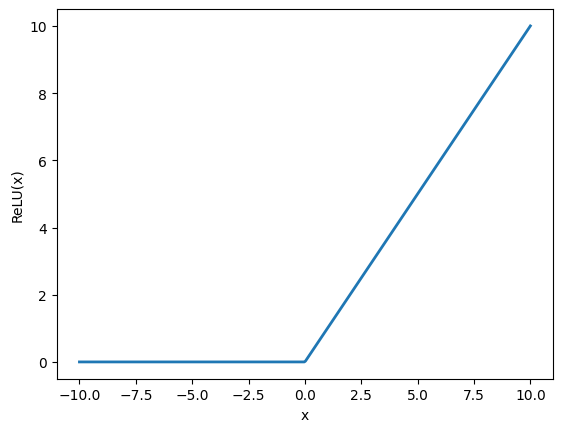
\includegraphics[width=\linewidth]{img/r5/relu.png}
		\caption{ReLU}
		\label{fig:wykres2}
	\end{subfigure}
	\hfill
	\begin{subfigure}[b]{0.45\textwidth}
		\centering
		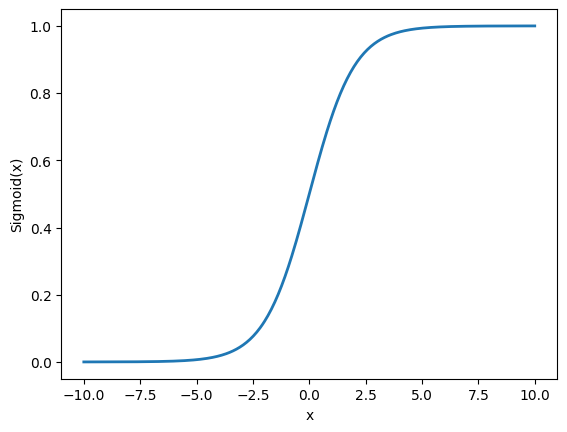
\includegraphics[width=\linewidth]{img/r5/sigmoid.png}
		\caption{Sigmoid}
		\label{Sigmoid}
	\end{subfigure}
\end{figure}

W prezentowanej architekturze zastosowano funkcję aktywacji ReLU w warstwach ukrytych, ze względu na jej wysoką efektywność obliczeniową oraz zdolność do wspomagania procesu uczenia głębokich sieci neuronowych. ReLU także minimalizuje problem zanikania gradientu.

W warstwie wyjściowej wykorzystano funkcję aktywacji sigmoidalną, której właściwości umożliwiają interpretację wyjścia modelu jako prawdopodobieństwa przynależności próbki do klasy pozytywnej. W związku z tym zastosowano jeden neuron w warstwie wyjściowej, którego wartość aktywacji reprezentuje stopień pewności modelu co do przypisania obserwacji do klasy pozytywnej.\\

Do optymalizacji wag modelu wykorzystano algorytm ADAM, który łączy zalety metod opartych na momentum oraz RMSProp. Optymalizator ten adaptacyjnie dostosowuje szybkość uczenia dla każdej z wag, uwzględniając zarówno średnie wartości gradientów z poprzednich epok, jak i ich skale\cite{kingma2014adam,ruder2016overview}.\\

Ze względu na rodzaj problemu, wybraną funkcją strat została binarna entropia krzyżowa. Funkcję tą można opisać przy pomocy wzoru:
\begin{equation}
	\mathcal{L}_{\text{avg}} = - \frac{1}{N} \sum_{i=1}^{N} \left( y_i \cdot \mathrm{log}(\hat{y}_i) + (1 - y_i) \cdot \mathrm{log}(1 - \hat{y}_i) \right)
\end{equation}

gdzie:
\begin{itemize}
	\item $N$  liczba próbek w zbiorze,
	\item $y_i$  prawdziwa etykieta $i$-tej próbki,
	\item $\hat{y}_i$  prawdopodobieństwo przypisane klasie pozytywnej dla $i$-tej próbki.
\end{itemize}
W eksperymencie przyjęto, że proces uczenia modelu będzie przebiegać przez 10 epok z rozmiarem partii równym 64. Zastosowano również dynamiczną regulacje kroku uczenia, w której początkowa wartość kroku uczenia wynosiła 0.001

Od piątej epoki zastosowano wykładniczy schemat zmniejszania kroku uczenia, zgodny z równaniem:	{
\begin{equation}
	Lr(epoka) =
	\begin{cases}
		Lr_0                          & \text{jeżeli } epoka < 5    \\
		Lr(epoka - 1) \times e^{-0.1} & \text{jeżeli } epoka \geq 5
	\end{cases}
\end{equation}
}
gdzie:
\begin{itemize}
	\item $Lr$ - krok uczenia
	\item $Lr_0$ - początkowy krok uczenia
\end{itemize}

W przypadku uczenia bezcechowego, zdecydowano się na przetestowanie czterech różnych architektur sieci neuronowych, zróżnicowanych pod względem rodzaju zastosowanych warstw.

Pierwsza architektura odpowiadała strukturze wykorzystanej w eksperymencie z uczeniem cechowym, co umożliwia bezpośrednie porównanie efektywności obu metod względem tego samego problemu klasyfikacyjnego.

Druga architektura wykorzystywała warstwy konwolucyjne jednowymiarowe , przeplatane warstwami MaxPooling1D, których zadaniem było redukowanie wymiarowości sygnału poprzez wybór wartości maksymalnej w lokalnym sąsiedztwie. Po zakończeniu ekstrakcji cech konwolucyjnych, zastosowano warstwę Flatten, która przekształca dane o strukturze wielowymiarowej do postaci wektora jednowymiarowego. Operacja ta jest niezbędna, aby możliwe było podłączenie kolejnych warstw gęstych, które przetwarzają wektor cech wygenerowany przez wcześniejsze warstwy konwolucyjne.

Trzecia rozważana architektura opiera się na dwóch sekwencyjnie połączonych warstwach typu LSTM, które są zdolne do modelowania zależności czasowych w sygnale. Warstwy te zostały uzupełnione o końcowe warstwy gęste, umożliwiające dokonanie klasyfikacji na podstawie reprezentacji uzyskanej z przetworzenia sekwencji czasowej.

Czwarta architektura stanowi połączenie podejść zastosowanych we wszystkich trzech wcześniejszych modelach. W pierwszym etapie wykorzystywane są warstwy konwolucyjne jednowymiarowe wraz z warstwami MaxPooling1D, których zadaniem jest lokalna ekstrakcja cech oraz redukcja wymiarowości danych. Wynikowy tensor jest następnie przekazywany do warstw LSTM, które modelują zależności czasowe. Ostatecznie, przetworzony wektor cech trafia do warstw gęstych, które realizują końcową klasyfikację.\\

We wszystkich opisanych architekturach przyjęto identyczny zestaw hiperparametrów procesu uczenia, jak w przypadku modelu uczącego się na danych cechowych. Dzięki temu możliwe było porównanie skuteczności różnych architektur przy zachowaniu spójnych warunków eksperymentalnych.\\

Zdecydowano się także, na przeprowadzenie procesu optymalizacji hiperparametrów modeli. Proces ten polegał na iteracyjnym zmianie hiperparametrów i testowaniu modeli. Całość procesu została wykonania przy pomocy bibloteki Optuna. Wykorzystuje ona strategie sekwencyjnej optymalizacji bayesowskiej. Metoda ta jest znacznie szybka niż wykorzystanie siatki parametrów lub losowego sprawdzania parametrów. Metoda ta, buduje modele probabilistyczne które uczą się procesu wybierania kolejnych zestawów hiperparametrów, balansując eksploracje nowych obszarów jak i ulepszanie znanych.\\


% \centering
% \caption{Testowane zakresy hiperparametrów}
% \label{tab:hiperparametry}

Nazwy hiperparametrów zamieszczone w tabeli \ref{tab:hiperparametry} zostały zaczerpnięte z dokumentacji technicznej wykorzystanej biblioteki \cite{sklearn_api}.\\

W przypadku algorytmu K najbliższych sąsiadów zdecydowano się na optymalizację dwóch kluczowych hiperparametrów. Pierwszym z nich była liczba sąsiadów k, wykorzystywana do predykcji klasy nowych próbek. W ramach procedury wyszukiwania optymalnych wartości badano wartości K z przedziału od 5 do 200. Drugim z optymalizowanych parametrów był parametr p w funkcji odległości Minkowskiego, który wpływa na sposób obliczania dystansu pomiędzy próbkami. W tym przypadku analizowano wartości całkowite z zakresu od 1 do 5.

Drzewo decyzyjne dysponuje większą liczbą hiperparametrów, które mogą podlegać procesowi optymalizacji. Parametr criterion odpowiada za sposób oceny jakości podziału danych w węzłach drzewa. Domyślną wartością tego parametru jest "gini", który opiera się na analizie proporcji klas. Alternatywnie, rozważono również wartość "entropy", która wykorzystuje entropię do określenia niepewności rozkładu klas w danym węźle.

Parametr max features definiuje maksymalną liczbę cech rozważanych podczas wyboru cechy, według której następuje podział. Natomiast parametry min samples split oraz min samples leaf kontrolują odpowiednio minimalną liczbę próbek wymaganą do dokonania podziału oraz minimalną liczbę próbek w liściu. Wartości tych trzech parametrów przeszukiwano w zbiorze liczb całkowitych od 1 do 20.

Ostatnim optymalizowanym parametrem było max depth, które określa maksymalną głębokość drzewa decyzyjnego, a tym samym maksymalną liczbę testów logicznych prowadzących od korzenia do liścia. Zakres wartości tego parametru obejmował liczby całkowite z przedziału od 3 do 20.\\


Las losowy dziedziczy wszystkie parametry drzewa decyzyjnego ze względu na swoje działanie oparte o równoległą naukę tych modeli. Dlatego parametry criterion, max features, min samples split, min samples leaf oraz max depth są optymalizowane w takich samych przedziałach jak w przypadku drzewa decyzyjnego.

Unikatowym hiperparametrem, który podlegał optymalizacji, jest n estimators, określający liczbę drzew decyzyjnych wchodzących w skład lasu losowego. Wartości tego parametru przeszukiwano w zbiorze liczb całkowitych z zakresu od 1 do 200.\\

Najważniejszym parametrem dla klasyfikatora SVM jest jądro, przy pomocy którego dokonywane są wewnętrzne przekształcenia przestrzeni cech. Zdecydowano się sprawdzić wszystkie cztery możliwości: linear, który oblicza iloczyn skalarny dwóch wektorów; poly, który rozszerza dane do przestrzeni wielomianowej; rbf, który wykorzystuje eksponentę kwadratu odległości euklidesowej; oraz sigmoid, który używa funkcji tangensa hiperbolicznego. Porównanie działania poszczególnych jąder przedstawia Rysunek~\ref{jadro_svm}.

Jądra wykorzystywane w metodzie SVM korzystają z dwóch wspólnych parametrów. Pierwszy z nich, gamma, określa wpływ pojedynczego punktu treningowego na przebieg granicy decyzyjnej. W niniejszym eksperymencie gamma może przyjmować dwie wartości: scale, która uwzględnia wariancję oraz liczbę cech, oraz auto, która opiera się wyłącznie na liczbie cech. Drugim parametrem jest C, który kontroluje siłę regularyzacji L2 podczas treningu. Parametr ten może przyjmować wartości zmiennoprzecinkowe z przedziału od $10^{-5}$ do $10^{5}$.

Ze względu na zróżnicowane działanie poszczególnych jąder, istnieją również parametry charakterystyczne dla niektórych z nich. Parametr degree określa rząd wielomianu, do którego rozwijane jest jądro poly, jego wartość będzie sprawdzana z liczb całkowitych od 2 do 5. Z kolei parametr coeff0 stanowi wartość przesunięcia dla jąder typu poly oraz sigmoid. Sprawdzanymi wartościami tego parametru będą liczby zmiennoprzecinkowe od -1 do 1. Jądra linear oraz rbf nie posiadają dodatkowych, charakterystycznych parametrów poza gamma oraz C.
\begin{table}[]
	\centering
	\caption{Testowane zakresy hiperparametrów}
	\label{tab:hiperparametry}
	\begin{tabular}{@{}ccc@{}}
		\toprule
		\textbf{Hiperparametr} & \textbf{Typ}      & \textbf{Wartości}          \\ \midrule
		\multicolumn{3}{c}{\textbf{KNN}}                                        \\ \midrule
		K                      & Liczba całkowita  & (5, 200)                   \\
		p                      & Liczba całkowita  & (1, 5)                     \\ \midrule
		\multicolumn{3}{c}{\textbf{DRZEWO DECYZYJNE}}                           \\ \midrule
		Criterion              & Kategoryczny      & gini, entropy              \\
		Max features           & Kategoryczny      & sqrt, log2, None           \\
		Min samples split      & Liczba całkowita  & (1, 20)                    \\
		Min samples leaf       & Liczba całkowita  & (1, 20)                    \\
		Max depth              & Liczba całkowita  & (3, 20)                    \\ \midrule
		\multicolumn{3}{c}{\textbf{LAS LOSOWY}}                                 \\ \midrule
		Criterion              & Kategoryczny      & gini, entropy              \\
		Max features           & Kategoryczny      & sqrt, log2, None           \\
		Min samples split      & Liczba całkowita  & (1, 20)                    \\
		Min samples leaf       & Liczba całkowita  & (1, 20)                    \\
		Max depth              & Liczba całkowita  & (3, 20)                    \\
		n estimators           & Liczba całkowita  & (1, 200)                   \\ \midrule
		\multicolumn{3}{c}{\textbf{SVM}}                                        \\ \midrule
		Kernel                 & Kategoryczny      & linear, poly, rbf, sigmoid \\
		Gamma                  & Kategoryczny      & scale, auto                \\
		Degree                 & Liczba całkowita  & (2, 5)                     \\
		Coef0                  & Liczba dziesiętna & (-1. 1)                    \\
		C                      & Liczba dziesiętna & ($10^{-5}$,  $10^{5}$)     \\ \bottomrule
	\end{tabular}
\end{table}

\newpage
\section{Walidacja wyników}
W celu oceny jakości predykcji modeli zastosowano dwie niezależne metody walidacji krzyżowej. TODO DOPISAĆ COŚ TUTAJ\\



\subsection{Walidacja holdout}
Pierwszą z użytych metod jest walidacja krzyżowa metodą holdout polega na jednorazowym podziale dostępnych danych na dwa rozłączne podzbiory: zbiór treningowy oraz zbiór testowy. Zbiór treningowy wykorzystywany jest do uczenia modelu, natomiast zbiór testowy służy do oceny jego zdolności generalizacji na nieznanych wcześniej danych. Najczęściej stosowaną proporcją podziału jest 80:20, gdzie 80\% danych trafia do zbioru treningowego, a pozostałe 20\% do testowego. Należy jednak podkreślić, że nie jest to wartość sztywno ustalona - wybór proporcji zależy od liczby dostępnych próbek oraz charakterystyki problemu.

W niektórych przypadkach, szczególnie przy zastosowaniu złożonych modeli wymagających doboru hiperparametrów, ze zbioru treningowego dodatkowo wydziela się zbiór walidacyjny. Wówczas zbiór treningowy dzielony jest na dwa podzbiory: zbiór uczący oraz zbiór walidacyjny. Zbiór walidacyjny służy do oceny jakości modelu podczas procesu dobór optymalnych hiperparametrów bez ryzyka przecieku informacji ze zbioru testowego. Jego wykorzystanie pozwala na kontrolowanie lepsze procesu uczenia, np. poprzez mechanizm wczesnego zatrzymania, który przerywa naukę modelu w momencie, gdy jakość predykcji na zbiorze walidacyjnym przestają się poprawiać, co ogranicza ryzyko przeuczenia.\\

{\LARGE
RYSUNEK}\\

Aby uniknać przecieku informacji, polegającego na tym, że model ma dostęp do danych testowych już na etapie treningu, z decydowano się użyć zbiorów X Y Z jako zbioru treningowego oraz zbioru ABC jako zbiór testujący. Przeciek taki prowadzi do sztucznego zawyżenia wartości metryk jakościowych, co z kolei fałszuje rzeczywistą skuteczność modelu w warunkach niezależnych od zbioru treningowego. W kontekście wdrożeniowym, gdzie modele są stosowane do danych nieobecnych podczas treningu, taki przeciek znacząco obniża przewidywaną skuteczność modeli. Z tego względu procedura walidacji została przeprowadzona w sposób rygorystyczny, z zachowaniem pełnej separacji danych treningowych i testowych.


\subsubsection*{Nauca cechowa}
\subsubsection*{Nauca bezcechowa}
\subsubsection*{Optymalizacjia hiperparametrów}
\newpage
\subsection{Walidacja K-Fold}
Drugą zastosowaną metodą oceny jakości modelu jest walidacja krzyżowa K-krotna. Procedura ta polega na K-krotnym podziale dostępnego zbioru danych na K zbliżonych rozmiarowo części, zwanych foldami. W każdej iteracji jeden z foldów pełni rolę zbioru testującego, natomiast pozostałe K-1 foldy służą do trenowania modelu. Proces ten jest powtarzany K razy, za każdym razem z innym foldem jako zestawem testowym. Dzięki temu każda obserwacja jest wykorzystana dokładnie raz do walidacji oraz K-1 razy do uczenia modelu. Zdecydowano się na wykonanie walidacji przy pomocy 5 foldów.\\

\begin{figure}[!h]
	\centering
	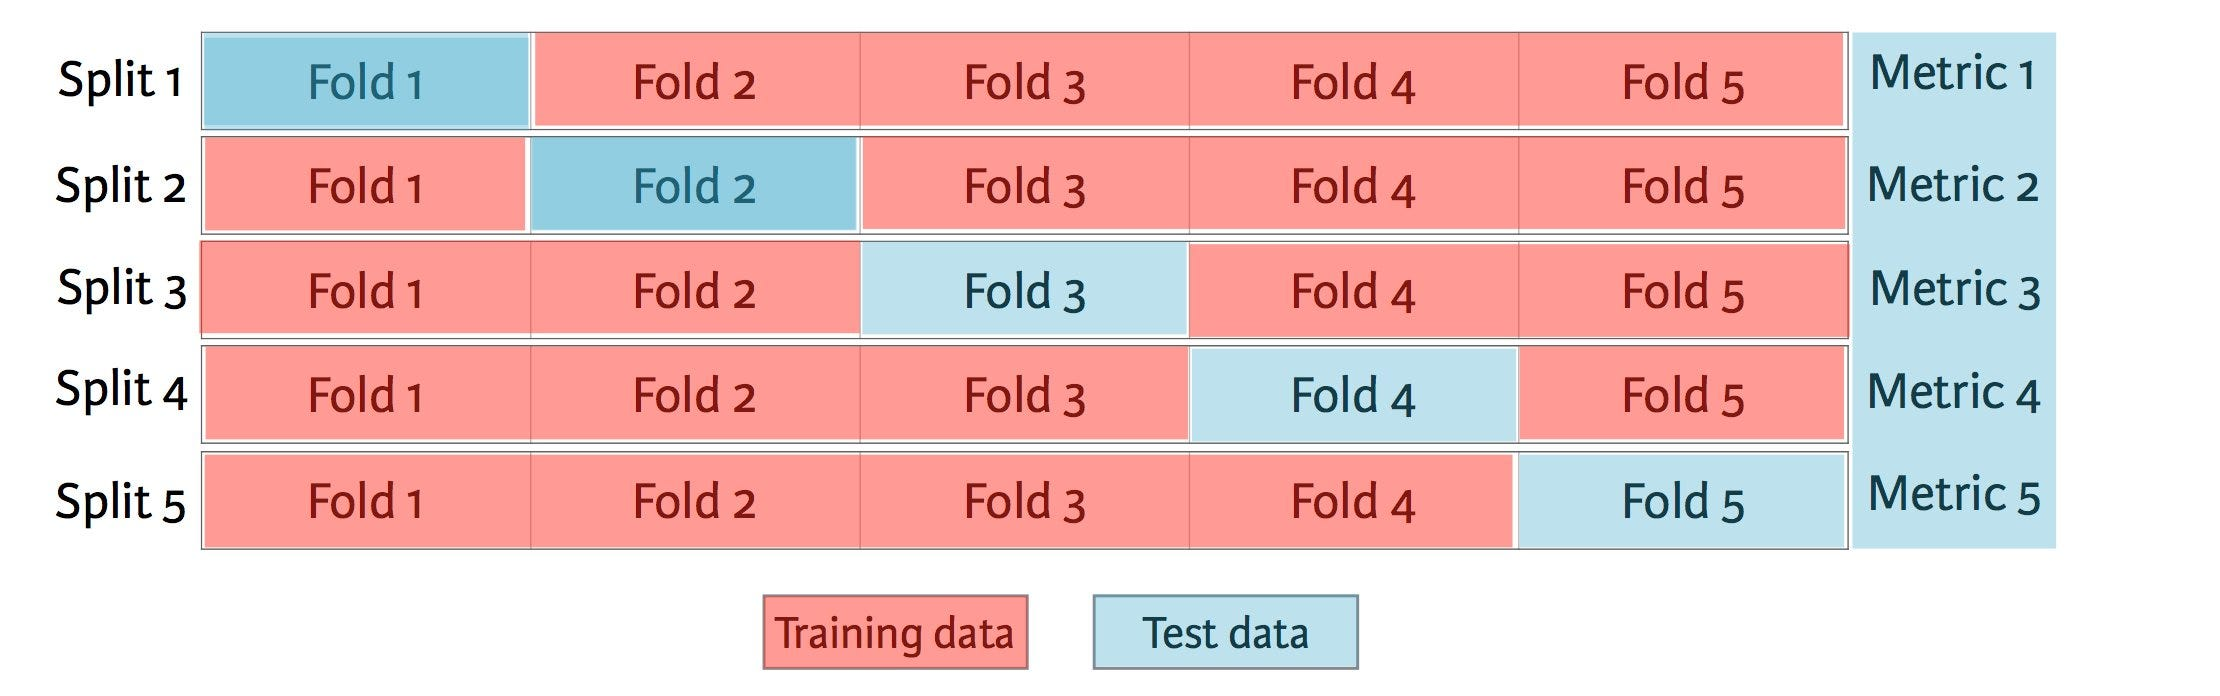
\includegraphics[width=1\textwidth]{img/r5/kfold.jpg}
	\caption{Wizualizacja walidacji Kfold\cite{allibhai2018holdout}}
	\label{fig:etykieta-rysunku}
\end{figure}

W przypadku zastosowania walidacji K-krotnej, w celu uniknięcia przecieku danych, zdecydowano się na ręczny przydział pacjentów do poszczególnych foldów. Dzięki temu próbki pochodzące od tego samego pacjenta nie występowały jednocześnie w zbiorze treningowym i walidacyjnym w żadnej z iteracji, co mogłoby prowadzić do sztucznego zawyżenia ocenianych metryk. Dodatkowo, w celu zapewnienia wiarygodności wyników, dane syntetyczne zostały wykluczone z procesu testowania, lecz były uwzględniane w trakcie uczenia modelu w każdej iteracji.\\

Ze względu na charakter metody walidacji krzyżowej K-Fold, w ramach jednego procesu walidacyjnego model jest  trenowany i testowany K razy. Skutkuje to otrzymaniem K niezależnych wyników dla każdej z metryk oceny modelu. W celu ich przejrzystej prezentacji zdecydowano się na przedstawienie rezultatów w postaci wartości średniej $\pm$ odchylenie standardowe. Taki sposób raportowania umożliwia nie tylko ocenę przeciętnej skuteczności modelu, ale również pozwala na analizę rozrzutu wyników między poszczególnymi foldami, dając pełniejszy obraz jakości modelu.
% Please add the following required packages to your document preamble:
% \usepackage{booktabs}


\newpage
\subsubsection*{Nauca cechowa}
\begin{table}[!h]
	\centering
	\caption{Wartości miar jakościowych dla nauki cechowej dla walidacji Kfold}
	\label{kfold_cechowa}
	\resizebox{\textwidth}{!}{
		\begin{tabular}{@{}>{\centering\arraybackslash}m{3.5cm}
			>{\centering\arraybackslash}m{2.5cm}
			>{\centering\arraybackslash}m{2.5cm}
			>{\centering\arraybackslash}m{2.5cm}
			>{\centering\arraybackslash}m{2.5cm}
			>{\centering\arraybackslash}m{2.5cm}@{}}
			\toprule
			                    & \textbf{Dokładność} & \textbf{Spec}   & \textbf{F-miara} & \textbf{nMCC}   & \textbf{FC}     \\
			\midrule
			\textbf{KNN}        & 0.83 $\pm$ 0.01     & 0.74 $\pm$ 0.03 & 0.87 $\pm$ 0.01  & 0.82 $\pm$ 0.01 & 0.82 $\pm$ 0.01 \\
			\textbf{\makecell{Drzewo                                                                                           \\Decyzyjne}} & 0.83 $\pm$ 0.01 & 0.77 $\pm$ 0.02 & 0.86 $\pm$ 0.00 & 0.83 $\pm$ 0.01 & 0.83 $\pm$ 0.01 \\
			\textbf{\makecell{Las                                                                                              \\Losowy}} & 0.84 $\pm$ 0.01 & 0.72 $\pm$ 0.03 & 0.87 $\pm$ 0.01 & 0.83 $\pm$ 0.01 & 0.82 $\pm$ 0.01 \\
			\textbf{Bayes}      & 0.50 $\pm$ 0.04     & 0.33 $\pm$ 0.28 & 0.57 $\pm$ 0.17  & 0.47 $\pm$ 0.02 & 0.48 $\pm$ 0.01 \\
			\textbf{SVM}        & 0.79 $\pm$ 0.01     & 0.61 $\pm$ 0.03 & 0.84 $\pm$ 0.01  & 0.78 $\pm$ 0.01 & 0.76 $\pm$ 0.01 \\
			\textbf{LLSVM}      & 0.78 $\pm$ 0.01     & 0.61 $\pm$ 0.02 & 0.83 $\pm$ 0.01  & 0.76 $\pm$ 0.01 & 0.75 $\pm$ 0.01 \\
			\textbf{XGBoost}    & 0.86 $\pm$ 0.01     & 0.81 $\pm$ 0.02 & 0.89 $\pm$ 0.01  & 0.86 $\pm$ 0.01 & 0.86 $\pm$ 0.01 \\
			\textbf{CatBoost}   & 0.86 $\pm$ 0.01     & 0.81 $\pm$ 0.02 & 0.89 $\pm$ 0.01  & 0.86 $\pm$ 0.01 & 0.86 $\pm$ 0.01 \\
			\textbf{LightBoost} & 0.85 $\pm$ 0.01     & 0.78 $\pm$ 0.03 & 0.88 $\pm$ 0.01  & 0.84 $\pm$ 0.01 & 0.84 $\pm$ 0.01 \\
			\textbf{\makecell{Sieć                                                                                             \\Neuronowa}} &0.82 ± 0.01 & 0.73 ± 0.05 & 0.85 ± 0.01& 0.81 ± 0.01 &0.81 ± 0.02 \\
			\bottomrule
		\end{tabular}
	}
\end{table}
Analizując dane przedstawione w tabeli \ref{kfold_cechowa}, można zaobserwować, że modele boostingowe najlepiej poradziły sobie z zadaniem wykrywania arytmii. Osiągnęły one najwyższe wartości we wszystkich miarach jakościowych. Modele XGBoost i CatBoost uzyskały identyczne wyniki, co wynika z faktu, że wykorzystują one zbliżone techniki modelowania zależności pomiędzy cechami a klasą. Charakteryzują się one wysokim poziomem równowagi pomiędzy precyzją a czułością, co potwierdza wysoka wartość F-miary. Jednocześnie nie tracą zdolności do wykrywania klasy zdrowych pacjentów, co potwierdza średnia swoistość na poziomie 81\%

Drugim najlepszym modelem pod względem wartości funkcji celu okazało się drzewo decyzyjne, którego wynik był zaledwie o 0,03 punktu procentowego niższy niż dla najlepszego modelu w przypadku funkcji celu, nMCC, F-miary oraz dokładności.

Las losowy, pomimo agregowania wielu drzew decyzyjnych, osiągnął nieco niższe wartości wskaźników jakościowych, z wyjątkiem F-miary, która była wyższa o 0,01 punktu procentowego. Może to sugerować, że model ten wymaga dokładniejszego strojenia hiperparametrów.

W przypadku klasyfikatora KNN wartości miar jakościowych były porównywalne do wyników uzyskanych przez las losowy.

Model SVM i LLSVM poradził sobie porównywalnie dobrze, ale SVM posiada każdy wskaźnij jakościowy nie gorszy niż LSSVM. Wciąż będać mniej wydajnym niż wcześnij omawiane modele.

Najgorzej z zadaniem wykrywania arytmii poradził sobie naiwny klasyfikator Bayesa. Uzyskał on najniższe wartości miar jakościowych: swoistość na poziomie 0.33 oraz nMCC wynoszące 0.47, co przełożyło się na ujemną wartość współczynnika MCC równą -0.06. Ponadto model ten cechował się największym rozrzutem wyników, podczas gdy odchylenie standardowe innych klasyfikatorów nie przekraczało 0.05, w tym przypadku osiągnęło nawet 0.28.

Sięc neuronowa, osiąngęła wyniki porównywalne z dobrymi klasyfikatorami, które są lepsze niż modele maszyn nośnych, ale gorsze niż las losowy, osiągajac wartość funkcji celu i nMCC na poziomie 0.81.

\begin{figure}[!h]
	\centering
	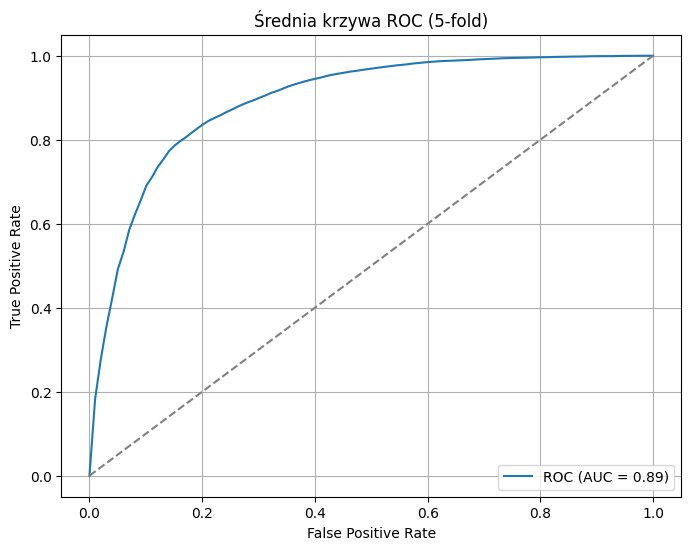
\includegraphics[width=0.7\textwidth]{img/roc_kfold_feature.png}
	\caption{Średnia krzywa ROC}
	\label{fig:etykieta-rysunku}
\end{figure}
Średnia krzywa ROC, wyznaczona na podstawie pięciu foldów walidacyjnych, wskazuje na bardzo dobrą zdolność modelu do klasyfikacji, osiągając wartość AUC równą 0,89. Krzywa ta wykazuje wyraźne wygięcie w kierunku lewego górnego narożnika wykresu oraz płaskie podejście do prawego górnego narożnika, co świadczy o wysokiej skuteczności klasyfikatora. Brakuje w niej fragmentów przebiegających blisko przekątnej. Krzywa jest ponadto stabilna i regularna, co dodatkowo potwierdza jej jakość.

\newpage
\subsubsection*{Nauca bezcechowa}

\begin{table}[!h]
	\centering
	\caption{Wartości miar jakościowych dla nauki bezcechowej dla walidacji Kfold}
	\label{kfold_bezcechowa}
	\resizebox{\textwidth}{!}{
		\begin{tabular}{@{}>{\centering\arraybackslash}m{3.5cm}
			>{\centering\arraybackslash}m{2.5cm}
			>{\centering\arraybackslash}m{2.5cm}
			>{\centering\arraybackslash}m{2.5cm}
			>{\centering\arraybackslash}m{2.5cm}
			>{\centering\arraybackslash}m{2.5cm}@{}}
			\toprule
			                  & \textbf{Dokładność} & \textbf{Spec}   & \textbf{F-miara} & \textbf{nMCC}   & \textbf{FC}     \\
			\midrule
			\textbf{Gęsta}    & 0.79 $\pm$ 0.01     & 0.61 $\pm$ 0.07 & 0.84 $\pm$ 0.01  & 0.77 $\pm$ 0.01 & 0.76 $\pm$ 0.02 \\
			\textbf{CNN}      & 0.78 $\pm$ 0.01     & 0.61 $\pm$ 0.07 & 0.83 $\pm$ 0.00  & 0.77 $\pm$ 0.01 & 0.75 $\pm$ 0.02 \\
			\textbf{LSTM}     & 0.63 $\pm$ 0.03     & 0.16 $\pm$ 0.13 & 0.76 $\pm$ 0.01  & 0.56 $\pm$ 0.07 & 0.53 $\pm$ 0.07 \\
			\textbf{CNN-LSTM} & 0.61 $\pm$ 0.00     & 0.00 $\pm$ 0.00 & 0.75 $\pm$ 0.00  & 0.50 $\pm$ 0.00 & 0.48 $\pm$ 0.00 \\
			\bottomrule
		\end{tabular}
	}
\end{table}

Analizując tabelę \ref{kfold_bezcechowa}, można zauważyć, że dwa pierwsze modele, sieć gęsta oraz CNN, poradziły sobie porównywalnie dobrze z zadaniem klasyfikacji, osiągając wartość znormalizowanego współczynnika korelacji równą 0,77. Pozostałe miary jakości również prezentują zadowalający poziom. Jedynym wskaźnikiem wyraźnie odbiegającym od reszty jest swoistość, która wyniosła zaledwie 0,61 i charakteryzowała się największym rozrzutem wartości.

Dodanie warstw LSTM doprowadziło do pogorszenia skuteczności klasyfikatorów. W skrajnym przypadku, sieć o architekturze CNN-LSTM klasyfikowała wszystkich pacjentów jako chorych, o czym świadczy zerowa wartość swoistości oraz nMCC wynoszący jedynie 0,50. Model ten uzyskał także najniższą wartość funkcji celu, równą zaledwie 0.48. Sieć LSTM bez warstw konwolucyjnych osiągnęła wyniki nieznacznie lepsze niż CNN-LSTM posiadajac swoistość na poziomie 0.16 oraz nMCC równe 0.56.\\

Analiza krzywych ROC przedstawionych na rysunku \ref{roc_bezcech} potwierdza wcześniej sformułowane wnioski. Można zaobserwować istotne różnice pomiędzy krzywymi ROC dla sieci gęstej (\ref{fig:dense}) i sieci konwolucyjnej (\ref{cnn}), a krzywymi dla modeli zawierających warstwy LSTM (\ref{lstm}) oraz CNN-LSTM (\ref{cnn-lstm}). Dwa pierwsze modele charakteryzują się krzywymi silnie wygiętymi w kierunku lewego górnego rogu wykresu oraz znacznym oddaleniem od przekątnej a ich pola pod krzywą wynoszą około 0.85.W przeciwieństwie do tego, krzywe ROC modeli zawierających warstwy LSTM są zbliżone do przekątnej wykresua ich wartości AUC oscylują wokół 0.5, co sugeruje niemal losowe prognozowanie klasy.



\begin{figure}[!ht]
	\centering
	\caption{Średnie krzywe ROC dla nauki bezcechowej}\
	\label{roc_bezcech}
	\begin{subfigure}[b]{0.49\textwidth}
		\centering
		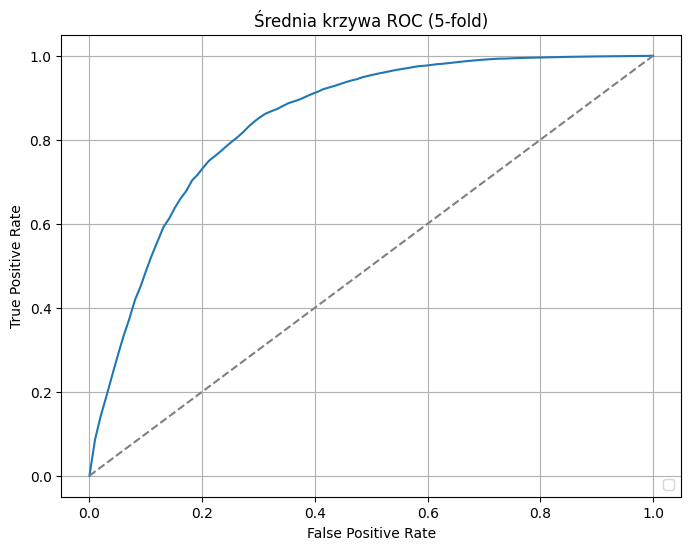
\includegraphics[width=\linewidth]{img/r5/kfold/bezcech_dense_roc_auc_0_85.png}
		\caption{Krzywa ROC sieci gęstej}
		\label{fig:dense}
	\end{subfigure}
	\hfill
	\begin{subfigure}[b]{0.49\textwidth}
		\centering
		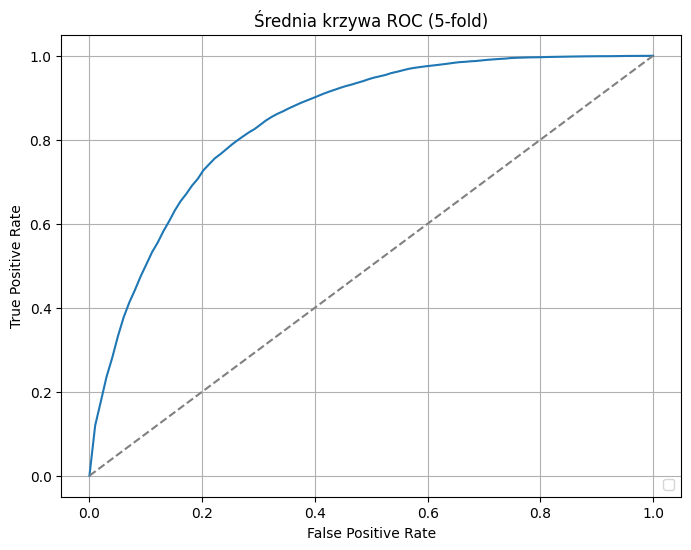
\includegraphics[width=\linewidth]{img/r5/kfold/bezcech_CNN_roc_auc_0_84.png}
		\caption{Krzywa ROC sieci CNN}
		\label{cnn}
	\end{subfigure}
	\begin{subfigure}[b]{0.49\textwidth}
		\centering
		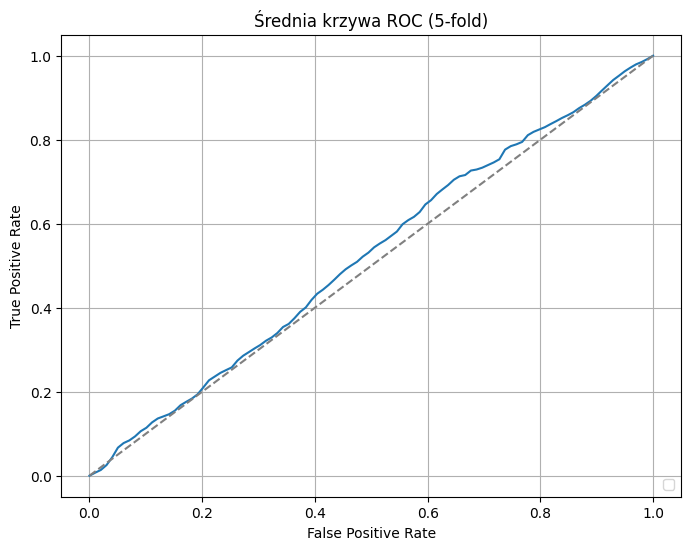
\includegraphics[width=\linewidth]{img/r5/kfold/bezcech_LSRM_roc_aug_0_52.png}
		\caption{Krzywa ROC sieci LSTM}
		\label{lstm}
	\end{subfigure}
	\begin{subfigure}[b]{0.49\textwidth}
		\centering
		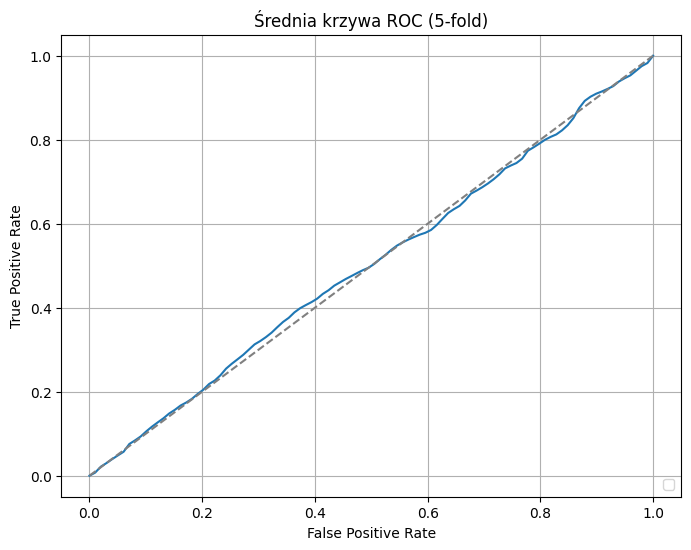
\includegraphics[width=\linewidth]{img/r5/kfold/bezcech_CNNLSTM_roc_aug_0_50.png}
		\caption{Krzywa ROC sieci CNN-LSTM}
		\label{cnn-lstm}
	\end{subfigure}
\end{figure}

\newpage
\subsubsection*{Optymalizacjia hiperparametrów}

\begin{table}[!h]
	\centering
	\caption{Wartości miar jakościowych po optymlizacji}
	\label{kfold_cechowa_opty}
	\resizebox{\textwidth}{!}{
		\begin{tabular}{@{}>{\centering\arraybackslash}m{3.5cm}
			>{\centering\arraybackslash}m{2.5cm}
			>{\centering\arraybackslash}m{2.5cm}
			>{\centering\arraybackslash}m{2.5cm}
			>{\centering\arraybackslash}m{2.5cm}
			>{\centering\arraybackslash}m{2.5cm}@{}}
			\toprule
			             & \textbf{Dokładność} & \textbf{Spec}   & \textbf{F-miara} & \textbf{nMCC}   & \textbf{FC}     \\
			\midrule
			\textbf{KNN} & 0.83 $\pm$ 0.00     & 0.73 $\pm$ 0.00 & 0.87 $\pm$ 0.00  & 0.82 $\pm$ 0.00 & 0.82 $\pm$ 0.00 \\
			\textbf{\makecell{Drzewo                                                                                    \\Decyzyjne}} & 0.83 $\pm$ 0.01 & 0.77 $\pm$ 0.02 & 0.86 $\pm$ 0.00 & 0.83 $\pm$ 0.01 & 0.83 $\pm$ 0.01 \\
			\textbf{\makecell{Las                                                                                       \\Losowy}} & 0.84 $\pm$ 0.01 & 0.72 $\pm$ 0.03 & 0.87 $\pm$ 0.01 & 0.83 $\pm$ 0.01 & 0.82 $\pm$ 0.01 \\
			\textbf{SVM} & 0.79 $\pm$ 0.01     & 0.61 $\pm$ 0.03 & 0.84 $\pm$ 0.01  & 0.78 $\pm$ 0.01 & 0.76 $\pm$ 0.01 \\
			\bottomrule
		\end{tabular}
	}
\end{table}
\section{Analiza wyników}

\chapter{Podsumowanie i wnioski}


% W całym dokumencie powinny znajdować się odniesienia do zawartych w nim ilustracji (rys. \ref{fig:2}).

% \begin{figure}
% 	\centering
% 	\begin{tikzpicture}
% 		\begin{axis}[
% 				y tick label style={
% 						/pgf/number format/.cd,
% 						fixed,   % po zakomentowaniu os rzednych jest indeksowana wykladniczo
% 						fixed zerofill, % 1.0 zamiast 1
% 						precision=1,
% 						/tikz/.cd
% 					},
% 				x tick label style={
% 						/pgf/number format/.cd,
% 						fixed,
% 						fixed zerofill,
% 						precision=2,
% 						/tikz/.cd
% 					}
% 			]
% 			\addplot [domain=0.0:0.1] {rnd};
% 		\end{axis}
% 	\end{tikzpicture}
% 	\caption{Wykres przebiegu funkcji.} % Podpis jest zawsze POD rysunkiem.
% 	\label{fig:2}
% \end{figure}


%%%%%%%%%%%%%%%%%%%%%
%% RYSUNEK Z PLIKU
%
%\begin{figure}
%\centering
%
\includegraphics[width=0.5\textwidth]{./politechnika_sl_logo_bw_pion_pl.pdf}
%\caption{Podpis rysunku zawsze pod rysunkiem.}
%\label{fig:etykieta-rysunku}
%\end{figure}
%Rys. \ref{fig:etykieta-rysunku} przestawia …
%%%%%%%%%%%%%%%%%%%%%
%
%%%%%%%%%%%%%%%%%%%%%
%% WIELE RYSUNKÓW 
%
%\begin{figure}
%\centering
%\begin{subfigure}{0.4\textwidth}
%    
\includegraphics[width=\textwidth]{./politechnika_sl_logo_bw_pion_pl.pdf}
%    \caption{Lewy górny rysunek.}
%    \label{fig:lewy-gorny}
%\end{subfigure}
%\hfill
%\begin{subfigure}{0.4\textwidth}
%    
\includegraphics[width=\textwidth]{./politechnika_sl_logo_bw_pion_pl.pdf}
%    \caption{Prawy górny rysunek.}
%    \label{fig:prawy-gorny}
%\end{subfigure}
%
%\begin{subfigure}{0.4\textwidth}
%    
\includegraphics[width=\textwidth]{./politechnika_sl_logo_bw_pion_pl.pdf}
%    \caption{Lewy dolny rysunek.}
%    \label{fig:lewy-dolny}
%\end{subfigure}
%\hfill
%\begin{subfigure}{0.4\textwidth}
%    
\includegraphics[width=\textwidth]{./politechnika_sl_logo_bw_pion_pl.pdf}
%    \caption{Prawy dolny rysunek.}
%    \label{fig:prawy-dolny}
%\end{subfigure}
%        
%\caption{Wspólny podpis kilku rysunków.}
%\label{fig:wiele-rysunkow}
%\end{figure}
%Rys. \ref{fig:wiele-rysunkow} przestawia wiele ważnych informacji, np. rys. \ref{fig:prawy-gorny} jest na prawo u góry.
%%%%%%%%%%%%%%%%%%%%%


% Tekst dokumentu powinien również zawierać odniesienia do tabel (tab. \ref{id:tab:wyniki}).

% \begin{table}
% 	\centering
% 	\caption{Opis tabeli nad nią.}
% 	\label{id:tab:wyniki}
% 	\begin{tabular}{rrrrrrrr}
% 		\toprule
% 		        & \multicolumn{7}{c}{metoda}                                                                                                                                  \\
% 		\cmidrule{2-8}
% 		        &                            &         & \multicolumn{3}{c}{alg. 3} & \multicolumn{2}{c}{alg. 4, $\gamma = 2$}                                                \\
% 		\cmidrule(r){4-6}\cmidrule(r){7-8}
% 		$\zeta$ & alg. 1                     & alg. 2  & $\alpha= 1.5$              & $\alpha= 2$                              & $\alpha= 3$ & $\beta = 0.1$ & $\beta = -0.1$ \\
% 		\midrule
% 		0       & 8.3250                     & 1.45305 & 7.5791                     & 14.8517                                  & 20.0028     & 1.16396       & 1.1365         \\
% 		5       & 0.6111                     & 2.27126 & 6.9952                     & 13.8560                                  & 18.6064     & 1.18659       & 1.1630         \\
% 		10      & 11.6126                    & 2.69218 & 6.2520                     & 12.5202                                  & 16.8278     & 1.23180       & 1.2045         \\
% 		15      & 0.5665                     & 2.95046 & 5.7753                     & 11.4588                                  & 15.4837     & 1.25131       & 1.2614         \\
% 		20      & 15.8728                    & 3.07225 & 5.3071                     & 10.3935                                  & 13.8738     & 1.25307       & 1.2217         \\
% 		25      & 0.9791                     & 3.19034 & 5.4575                     & 9.9533                                   & 13.0721     & 1.27104       & 1.2640         \\
% 		30      & 2.0228                     & 3.27474 & 5.7461                     & 9.7164                                   & 12.2637     & 1.33404       & 1.3209         \\
% 		35      & 13.4210                    & 3.36086 & 6.6735                     & 10.0442                                  & 12.0270     & 1.35385       & 1.3059         \\
% 		40      & 13.2226                    & 3.36420 & 7.7248                     & 10.4495                                  & 12.0379     & 1.34919       & 1.2768         \\
% 		45      & 12.8445                    & 3.47436 & 8.5539                     & 10.8552                                  & 12.2773     & 1.42303       & 1.4362         \\
% 		50      & 12.9245                    & 3.58228 & 9.2702                     & 11.2183                                  & 12.3990     & 1.40922       & 1.3724         \\
% 		\bottomrule
% 	\end{tabular}
% \end{table}


%\chapter{[Przedmiot pracy]}
%
%\begin{itemize}
%\item  Jak ja rozwiązuję problem?
%\begin{itemize}
%\item rozwiązanie zaproponowane przez dyplomanta
%\item analiza teoretyczna rozwiązania
%\item uzasadnienie wyboru zastosowanych metod, algorytmów, narzędzi
%\end{itemize}
%\end{itemize}


% TODO
%
% 
%
%Rozdział przedstawia przeprowadzone badania. Jest to zasadnicza część i~musi wyraźnie dominować w~pracy.
%Badania i analizę wyników należy przeprowadzić, tak jak jest przyjęte w środowisku naukowym (na przykład korzystanie z danych benchmarkowych, walidacja krzyżowa, zapewnienie powtarzalności testów itd). 
%
%\section{Metodyka badań}
%
%\begin{itemize}
%\item opis metodyki badań
%\item opis stanowiska badawczego (opis interfejsu aplikacji badawczych -- w~załączniku)
%\end{itemize}
%
%
%\section{Zbiory danych}
%
%\begin{itemize}
%\item opis danych
%\end{itemize}
%
%
%\section{Wyniki}
%
%\begin{itemize}
%\item prezentacja wyników, opracowanie i poszerzona dyskusja  wyników, wnioski
%\end{itemize}
%
% 
%\begin{table}
%\centering
%\caption{Opis tabeli nad nią.}
%\label{id:tab:wyniki}
%\begin{tabular}{rrrrrrrr}
%\toprule
%	         &                                     \multicolumn{7}{c}{metoda}                                      \\
%	         \cmidrule{2-8}
%	         &         &         &        \multicolumn{3}{c}{alg. 3}        & \multicolumn{2}{c}{alg. 4, $\gamma = 2$} \\
%	         \cmidrule(r){4-6}\cmidrule(r){7-8}
%	$\zeta$ &     alg. 1 &   alg. 2 & $\alpha= 1.5$ & $\alpha= 2$ & $\alpha= 3$ &   $\beta = 0.1$  &   $\beta = -0.1$ \\
%\midrule
%	       0 &  8.3250 & 1.45305 &       7.5791 &    14.8517 &    20.0028 & 1.16396 &                       1.1365 \\
%	       5 &  0.6111 & 2.27126 &       6.9952 &    13.8560 &    18.6064 & 1.18659 &                       1.1630 \\
%	      10 & 11.6126 & 2.69218 &       6.2520 &    12.5202 &    16.8278 & 1.23180 &                       1.2045 \\
%	      15 &  0.5665 & 2.95046 &       5.7753 &    11.4588 &    15.4837 & 1.25131 &                       1.2614 \\
%	      20 & 15.8728 & 3.07225 &       5.3071 &    10.3935 &    13.8738 & 1.25307 &                       1.2217 \\
%	      25 &  0.9791 & 3.19034 &       5.4575 &     9.9533 &    13.0721 & 1.27104 &                       1.2640 \\
%	      30 &  2.0228 & 3.27474 &       5.7461 &     9.7164 &    12.2637 & 1.33404 &                       1.3209 \\
%	      35 & 13.4210 & 3.36086 &       6.6735 &    10.0442 &    12.0270 & 1.35385 &                       1.3059 \\
%	      40 & 13.2226 & 3.36420 &       7.7248 &    10.4495 &    12.0379 & 1.34919 &                       1.2768 \\
%	      45 & 12.8445 & 3.47436 &       8.5539 &    10.8552 &    12.2773 & 1.42303 &                       1.4362 \\
%	      50 & 12.9245 & 3.58228 &       9.2702 &    11.2183 &    12.3990 & 1.40922 &                       1.3724 \\
%\bottomrule
%\end{tabular}
%\end{table}  
%
%
% 
%\begin{figure}
%\centering
%\begin{tikzpicture}
%\begin{axis}[
%    y tick label style={
%        /pgf/number format/.cd,
%            fixed,   % po zakomentowaniu os rzednych jest indeksowana wykladniczo
%            fixed zerofill, % 1.0 zamiast 1
%            precision=1,
%        /tikz/.cd
%    },
%    x tick label style={
%        /pgf/number format/.cd,
%            fixed,
%            fixed zerofill,
%            precision=2,
%        /tikz/.cd
%    }
%]
%\addplot [domain=0.0:0.1] {rnd};
%\end{axis} 
%\end{tikzpicture}
%\caption{Podpis rysunku po rysunkiem.}
%\label{fig:2}
%\end{figure}
%
%
%\begin{figure}
%\begin{lstlisting}
%if (_nClusters < 1)
%	throw std::string ("unknown number of clusters");
%if (_nIterations < 1 and _epsilon < 0)
%	throw std::string ("You should set a maximal number of iteration or minimal difference -- epsilon.");
%if (_nIterations > 0 and _epsilon > 0)
%	throw std::string ("Both number of iterations and minimal epsilon set -- you should set either number of iterations or minimal epsilon.");
%\end{lstlisting}
%\caption{Przykład pseudokodu}
%\end{figure}


% TODO



%\begin{itemize}
%\item Jaki problem rozwiązałæm?
%\item Jak ten problem rozwiązałæm?
%\item Jakie są dobre i słabe strony mojego rozwiązania?
%\item Czy mogę sformułować jakieś rekomendacje?
%\end{itemize}

\begin{itemize}
	\item syntetyczny opis wykonanych prac
	\item wnioski
	\item możliwość rozwoju, kontynuacji prac, potencjalne nowe kierunki
	\item Czy cel pracy zrealizowany?
\end{itemize}



\backmatter

%\bibliographystyle{plplain}  % bibtex
%\bibliography{biblio} % bibtex
\printbibliography           % biblatex
\addcontentsline{toc}{chapter}{Bibliografia}

\begin{appendices}

	% TODO


	% TODO
	\chapter{Spis skrótów i symboli}

	\begin{itemize}
		\item[PPG] Sygnał fotopletyzmograficzny
		\item[$\bar{x}$] Średnia wartość sygnału
		\item[$\sigma$] Odchylenie standardowe
		\item[H] Entropie Shannona
		\item[E] Energia
		\item[RMSSD] Pierwiastek średniokwadratowy różnic
		\item[kurt] Kurtoza widma
		\item[MVC] model -- widok -- kontroler (ang. \english{model--view--controller})
		\item[$\mu$] stopnień przyleżności do zbioru
		\item[$\mathbb{E}$] zbiór krawędzi grafu
		\item[$\mathcal{L}$] transformata Laplace'a
	\end{itemize}

	% TODO
	\chapter{Lista dodatkowych plików, uzupełniających tekst pracy}

	W systemie do pracy dołączono dodatkowe pliki zawierające:
	\begin{itemize}
		\item źródła programu,
		\item zbiory danych użyte w~eksperymentach,
		\item film pokazujący działanie opracowanego oprogramowania lub zaprojektowanego i wykonanego urządzenia,
		\item itp.
	\end{itemize}


	\listoffigures
	\addcontentsline{toc}{chapter}{Spis rysunków}
	\listoftables
	\addcontentsline{toc}{chapter}{Spis tabel}

\end{appendices}

\end{document}


%% Finis coronat opus.

